\documentclass{beamer}

\mode<presentation>
{
  \usetheme{Frankfurt}
  \usecolortheme{seahorse}
  \setbeamercovered{invisible}
  \usefonttheme{structurebold}
}

\usepackage[english]{babel}
\usepackage[latin1]{inputenc}
\usepackage{times}
\usepackage[T1]{fontenc} 
% Or whatever. Note that the encoding and the font should match. If T1
% does not look nice, try deleting the line with the fontenc.
\usepackage{amsmath}

\newcommand{\linespace}{\vskip 0.25cm}

\definecolor{MyForestGreen}{rgb}{0,0.7,0} 
\newcommand{\tableemph}[1]{{#1}}
\newcommand{\tablewin}[1]{\tableemph{#1}}
\newcommand{\tablemid}[1]{\tableemph{#1}}
\newcommand{\tablelose}[1]{\tableemph{#1}}

\definecolor{MyLightGray}{rgb}{0.6,0.6,0.6}
\newcommand{\tabletie}[1]{\color{MyLightGray} {#1}}
% The text in square brackets is the short version of your title and will be used in the
% header/footer depending on your theme.
\title[AAD through GPHH]{Automating Algorithm Design through\\Genetic Programming Hyper-Heuristicss}

% Sub-titles are optional - uncomment and edit the next line if you want one.
% \subtitle{Why does sub-tree crossover work?} 

% The text in square brackets is the short version of your name(s) and will be used in the
% header/footer depending on your theme.
\author[Browning]{Elsa Browning}

% The text in square brackets is the short version of your institution and will be used in the
% header/footer depending on your theme.
\institute[U of Minn, Morris]
{
  Division of Science and Mathematics \\
  University of Minnesota, Morris \\
  Morris, Minnesota, USA
}

% The text in square brackets is the short version of the date if you need that.
\date[April '17] % (optional)
{April 15, 2017\\ Morris, MN}

% Delete this, if you do not want the table of contents to pop up at
% the beginning of each subsection:
\AtBeginSection[]
{
  \begin{frame}<beamer>
    \frametitle{Outline}
    \tableofcontents[currentsection, hideothersubsections]
  \end{frame}
}

\begin{document}

\begin{frame}
  \titlepage
\end{frame}

% For a 20-25 minute senior seminar talk you probably want something like:
% - Two or three major sections (other than the summary).
% - At *most* three subsections per section.
% - Talk about 30s to 2min per frame. So there should probably be between
%   15 and 30 frames, all told.

\section*{Overview}

\subsection*{What does the title mean?}

\begin{frame}
	\frametitle{What does the title mean?}
	\begin{columns}
		\begin{column}{0.68\textwidth}
			\begin{itemize}
				\item Reducing the human component in algorithm design
				\linespace
				\item \pause More work at the beginning, more possibilities
				\linespace
				\item \pause Genetic programming hyper-heuristics as a method to the madness
			\end{itemize}
		\end{column}
		\begin{column}{0.32\textwidth}
			\pause[0]
			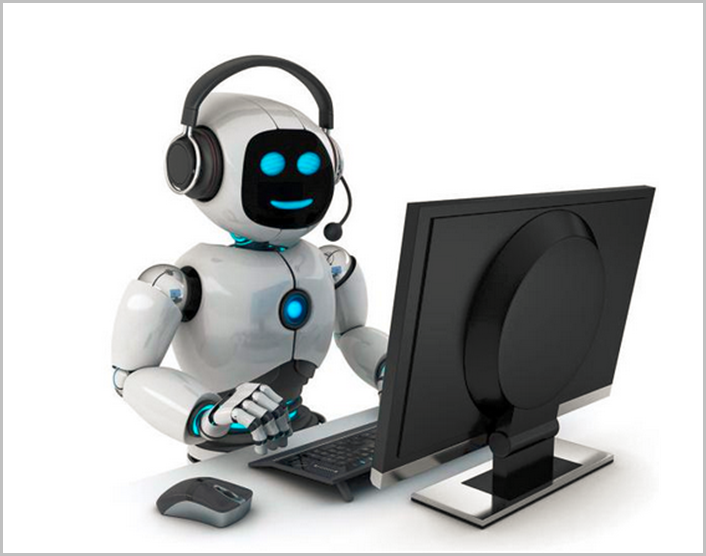
\includegraphics[height=.90\textwidth]{Illustrations/computer_robot.PNG}
			\\
			\only{\tiny{\url{https://scratch.mit.edu/discuss/m/topic/200574/} }}
		\end{column}
	\end{columns}
\end{frame}

\subsection*{Outline}

\begin{frame}
	\frametitle{Outline}
	\tableofcontents[hideallsubsections]
\end{frame}

\section[Background]{Background}

\subsection{Evolutionary Computation}

\begin{frame}
	\frametitle{Evolutionary Computation}
	\centering
	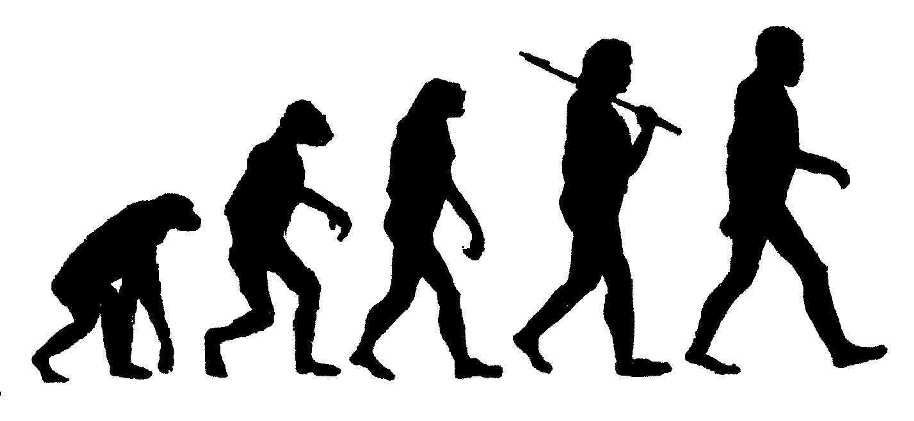
\includegraphics[width=.6\textwidth]{Illustrations/evolution.jpg}
	\\
	\only{\tiny{\url{https://www.spigotmc.org/attachments/evolution-jpg.137048/} }}
	\large
	\begin{itemize}
		\item Subfield of Artificial Intelligence
		\pause
		\item Algorithms based on biological evolution
		\pause
		\item Uses lots of terminology from biology, doesn't always mean same thing as term means in biology.
	\end{itemize}
\end{frame}

\begin{frame}
	\frametitle{Evolutionary Computation~--~Terminology}
	\begin{columns}
		\begin{column}{0.7\textwidth}
			\begin{itemize}
				\item \textbf{Individual}~--~a potential solution to a problem (or set of problems)
				\linespace
				\linespace
				\linespace
				\pause
				\item \textbf{Population}~--~a group of individuals
				\linespace
				\linespace
				\linespace
				\pause
				\item \textbf{Fit}~--~how well suited an individual is at solving a problem
				\linespace
				\linespace
				\linespace
				\pause
				\item \textbf{Fitness Test}~--~a set of tests to determine how fit an individual is.
			\end{itemize}
		\end{column}
		\begin{column}{0.3\textwidth}
			\pause[0]
			
\includegraphics[width=.25\textwidth]{Illustrations/individual.PDF}
			\linespace
			\pause[2]
			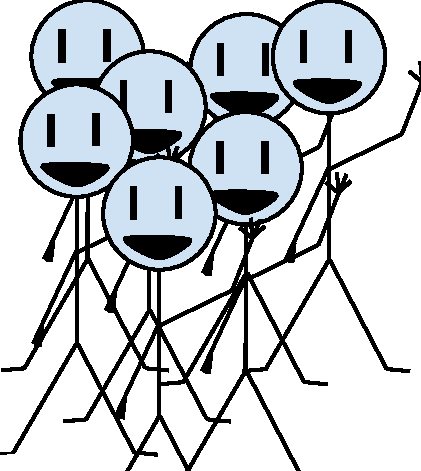
\includegraphics[height=.4\textwidth]{Illustrations/population.PDF}
			\linespace
			\pause[3]
			
\includegraphics[height=.5\textwidth]{Illustrations/fit.PDF}
			\linespace
			\pause[4]
			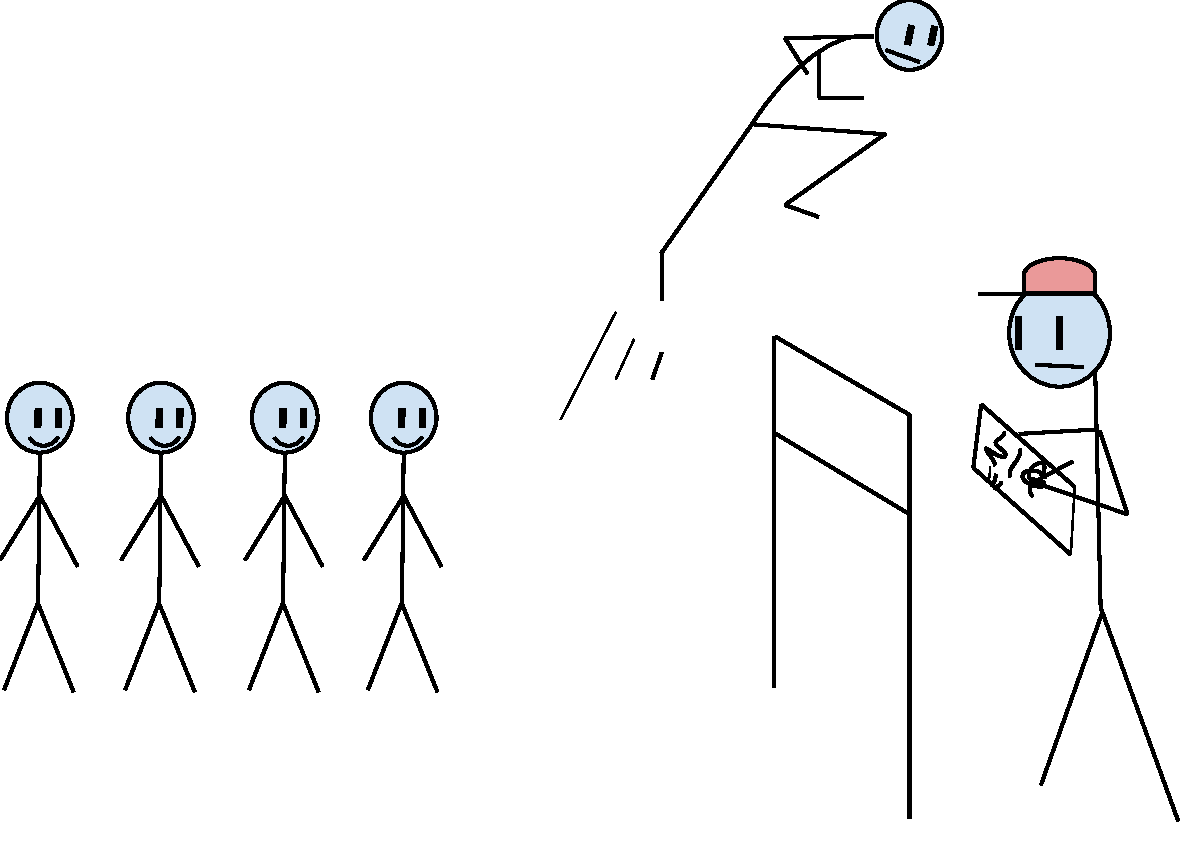
\includegraphics[height=.7\textwidth]{Illustrations/fitness_test.PDF}
		\end{column}
		\end{columns}
\end{frame}

\begin{frame}
	\frametitle{Evolutionary Computation~--~Terminology}
	\begin{itemize}
		\item \textbf{Mutation}~--~an insertion, deletion, or small change in the code of an individual, creating a new individual
		\linespace
		\pause
		\item \textbf{Sexual reproduction}~--~when two or more individuals are munged together to create a new individual
		\linespace
		\pause
		\item \textbf{Generation}~--~a population of individuals
		\pause
		\linespace
		\item \textbf{Global optima}~--~best solution (or solutions) possible
	\end{itemize}
\end{frame}

\begin{frame}
	\frametitle{Evolutionary Computation~--~Terminology}
	If individual A experiences a mutation to create individual B, then:
	\begin{columns}
		\begin{column}{.6\textwidth}
			\begin{itemize}
				\pause
				\item \textbf{Parent}~--~Individual A
				\linespace
				\linespace
				\linespace
				\linespace
				\pause
				\item \textbf{Child}~--~Individual B
			\end{itemize}
		\end{column}
		\begin{column}{.4\textwidth}
			\pause[2]
			
\includegraphics[height=.4\textwidth]{Illustrations/individual.PDF}
			\linespace
			\pause[3]
			
\includegraphics[height=.6\textwidth]{Illustrations/child.PDF}
		\end{column}
	\end{columns}
\end{frame}

\subsection{Genetic Programming}

\begin{frame}
	\frametitle{Genetic Programming}
	A family of algorithms in Evolutionary Computation that uses biological techniques to create programs to solve computational problems.
\end{frame}

\begin{frame}
	\frametitle{Genetic Programming}
	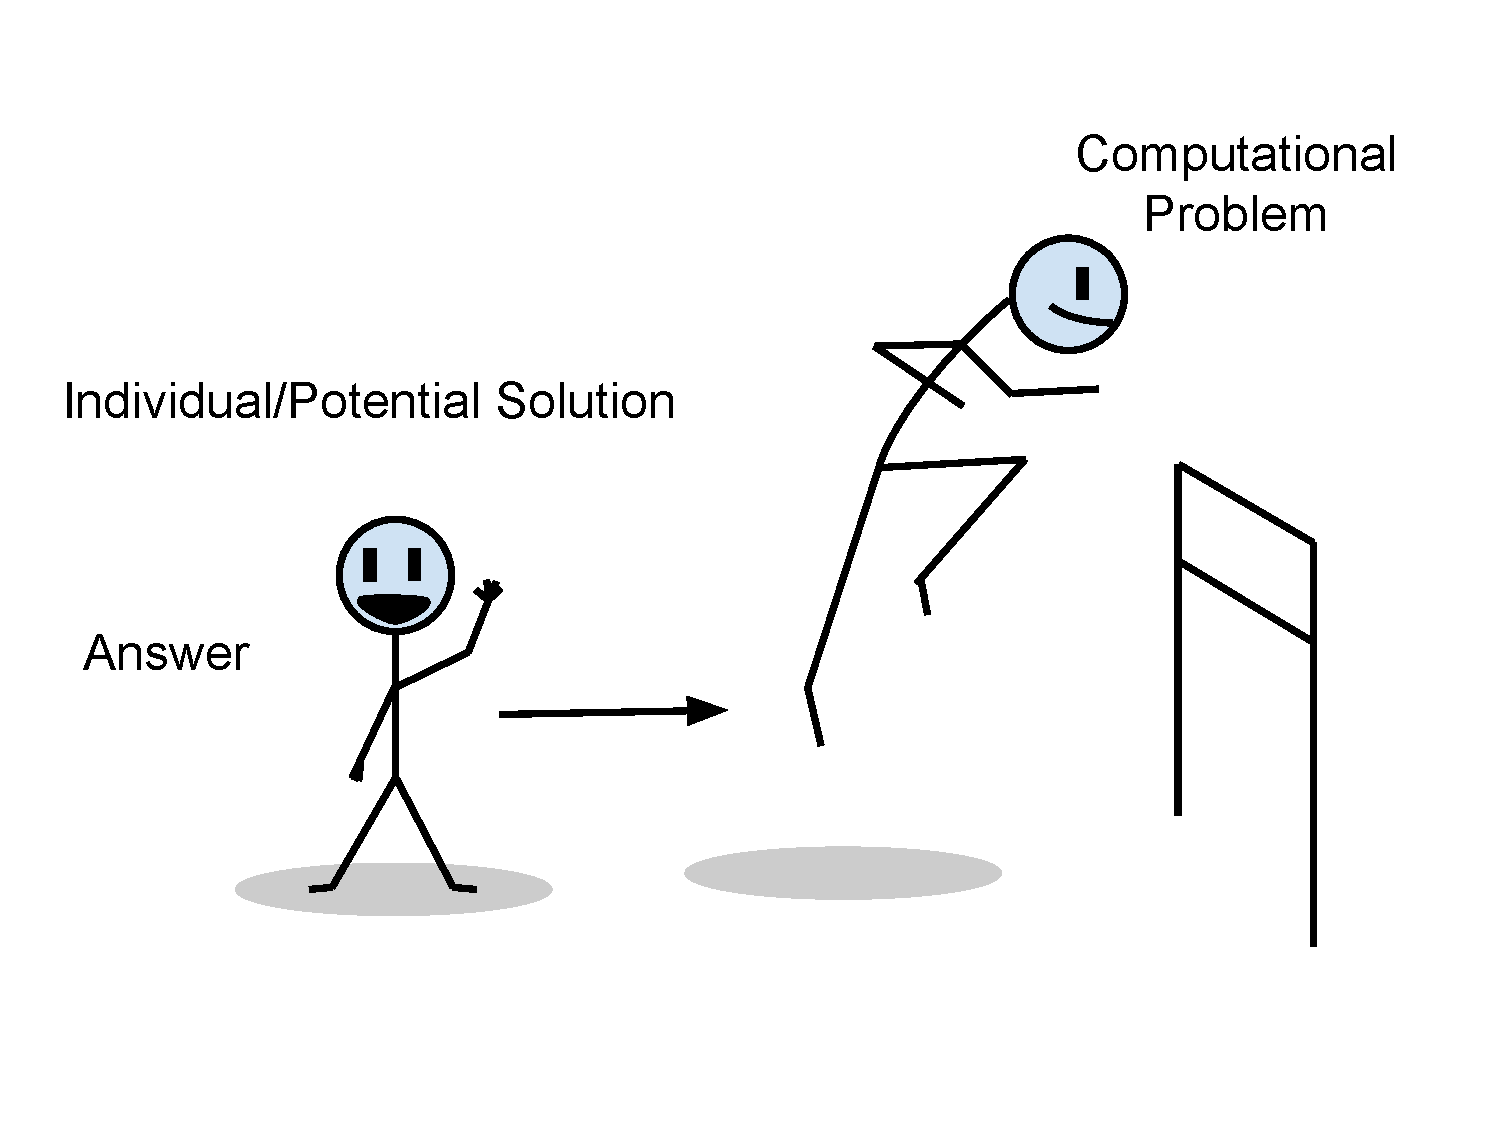
\includegraphics[height=.9\textheight]{Illustrations/gp_1.PDF}
\end{frame}
\begin{frame}
	\frametitle{Genetic Programming}
	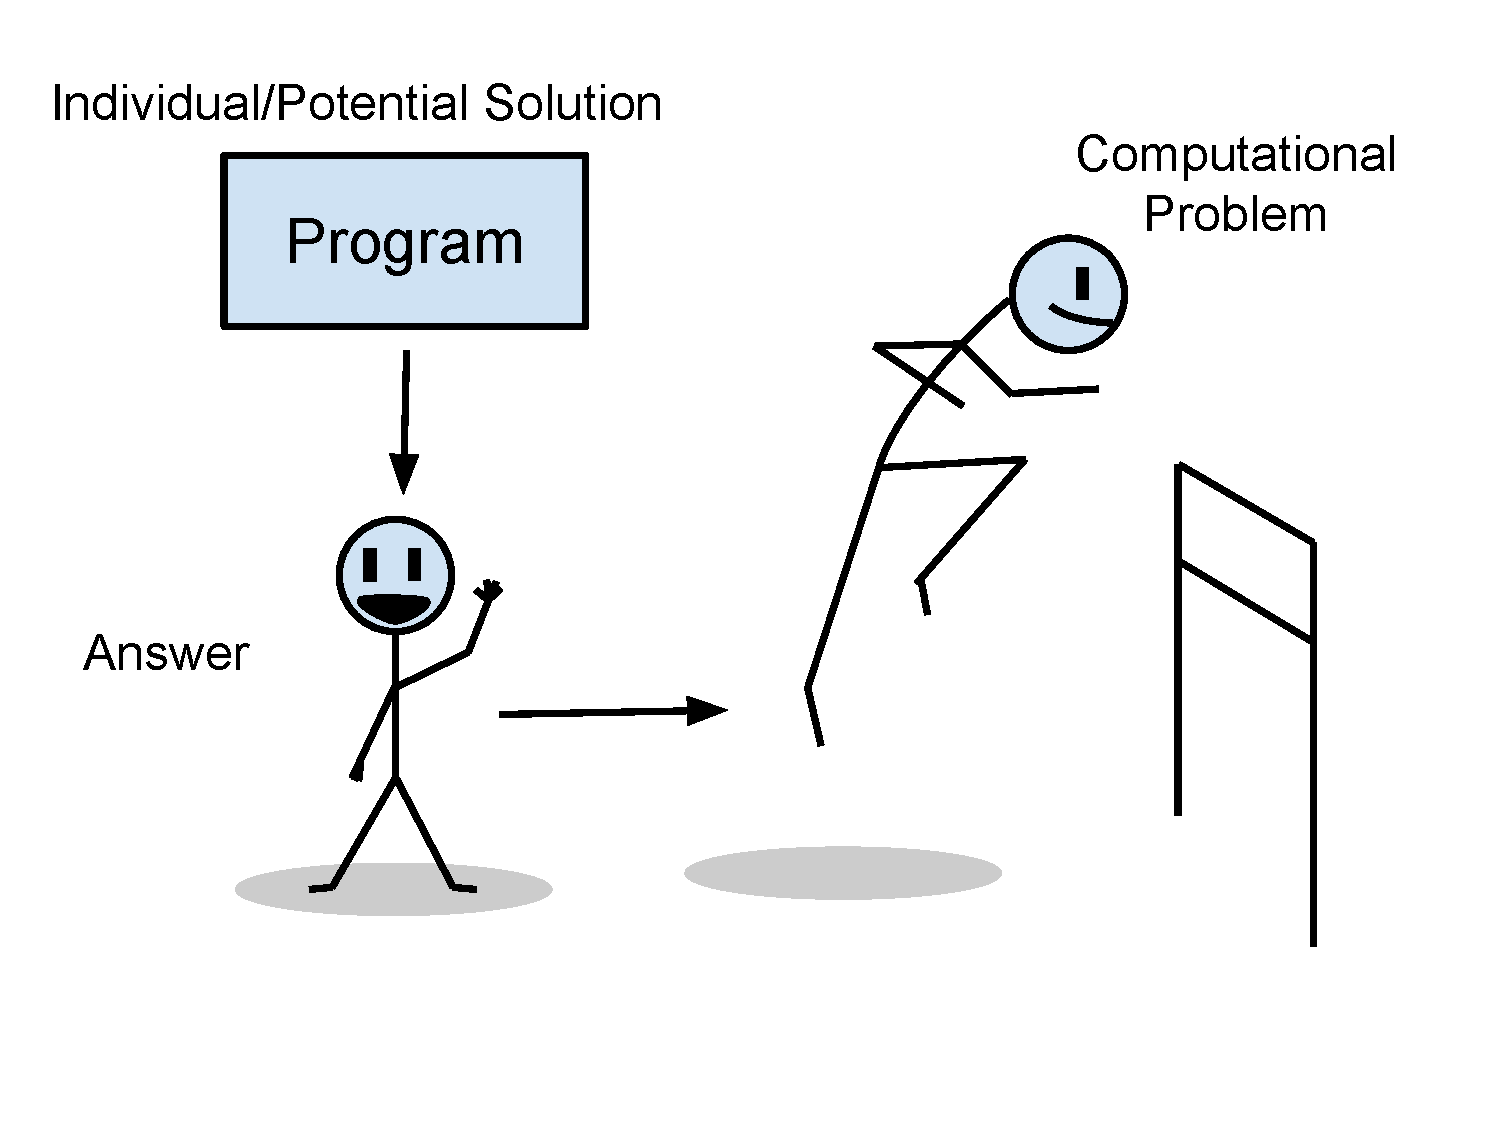
\includegraphics[height=.9\textheight]{Illustrations/gp_2.PDF}
\end{frame}
\begin{frame}
	\frametitle{Genetic Programming}
	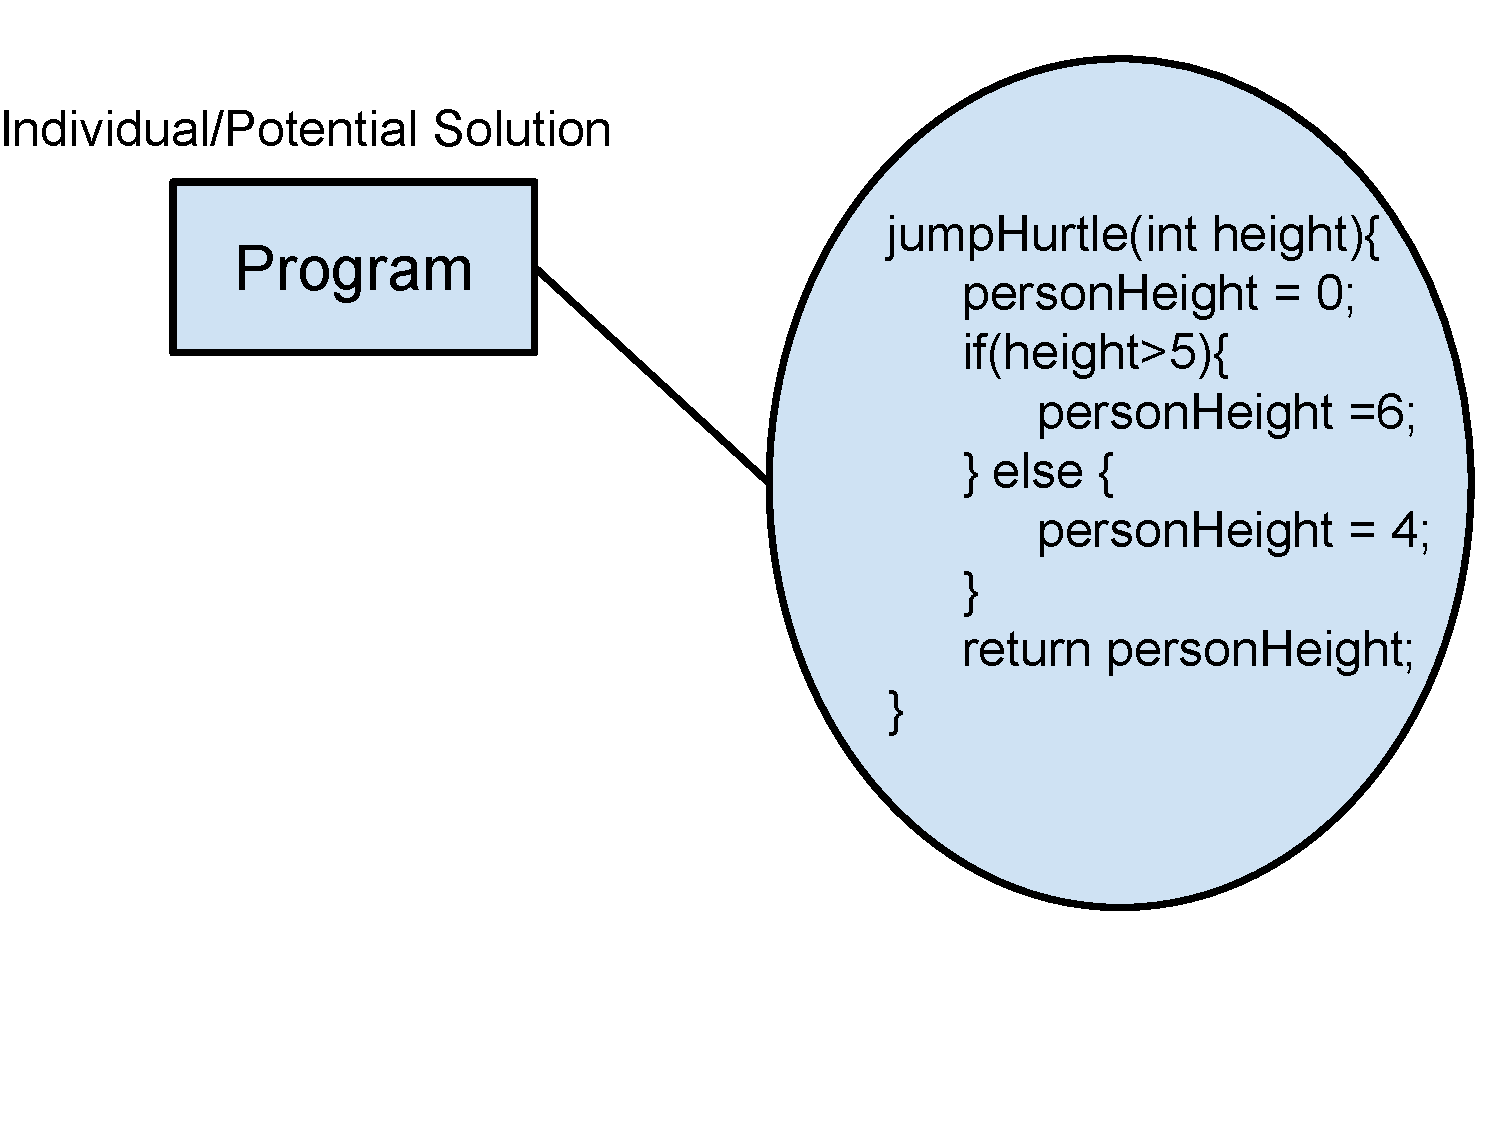
\includegraphics[height=.9\textheight]{Illustrations/gp_3.PDF}
\end{frame}
\begin{frame}
	\frametitle{Genetic Programming}
	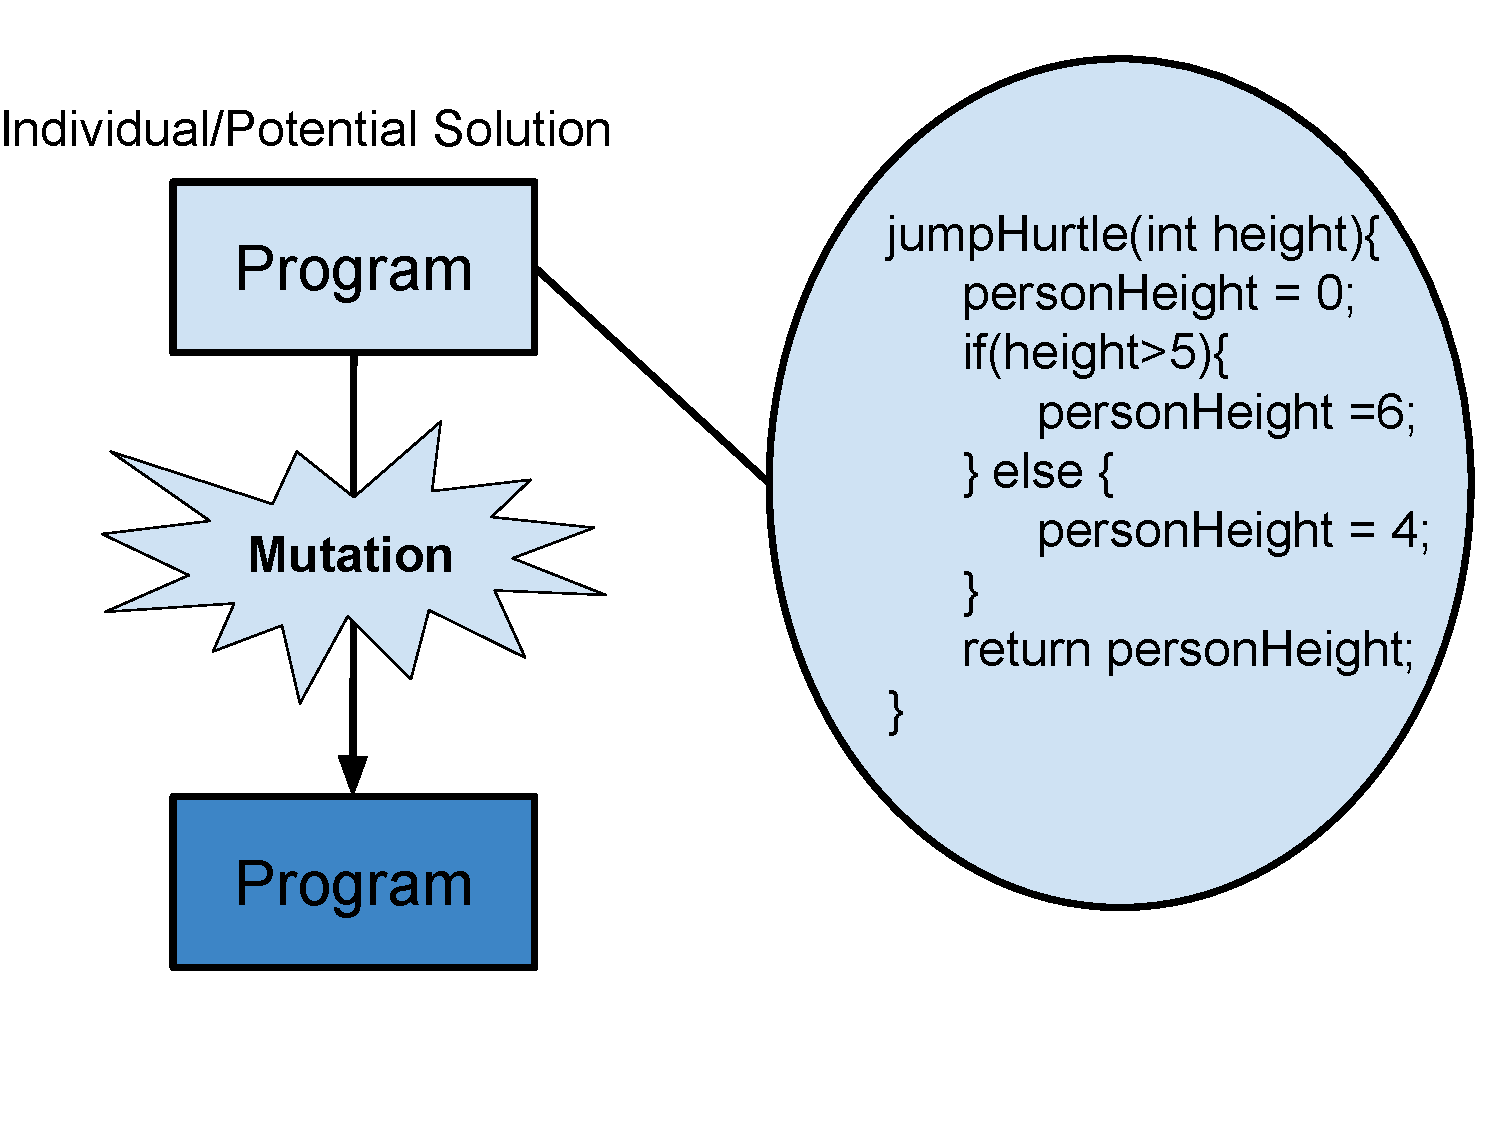
\includegraphics[height=.9\textheight]{Illustrations/gp_4.PDF}
\end{frame}
\begin{frame}
	\frametitle{Genetic Programming}
	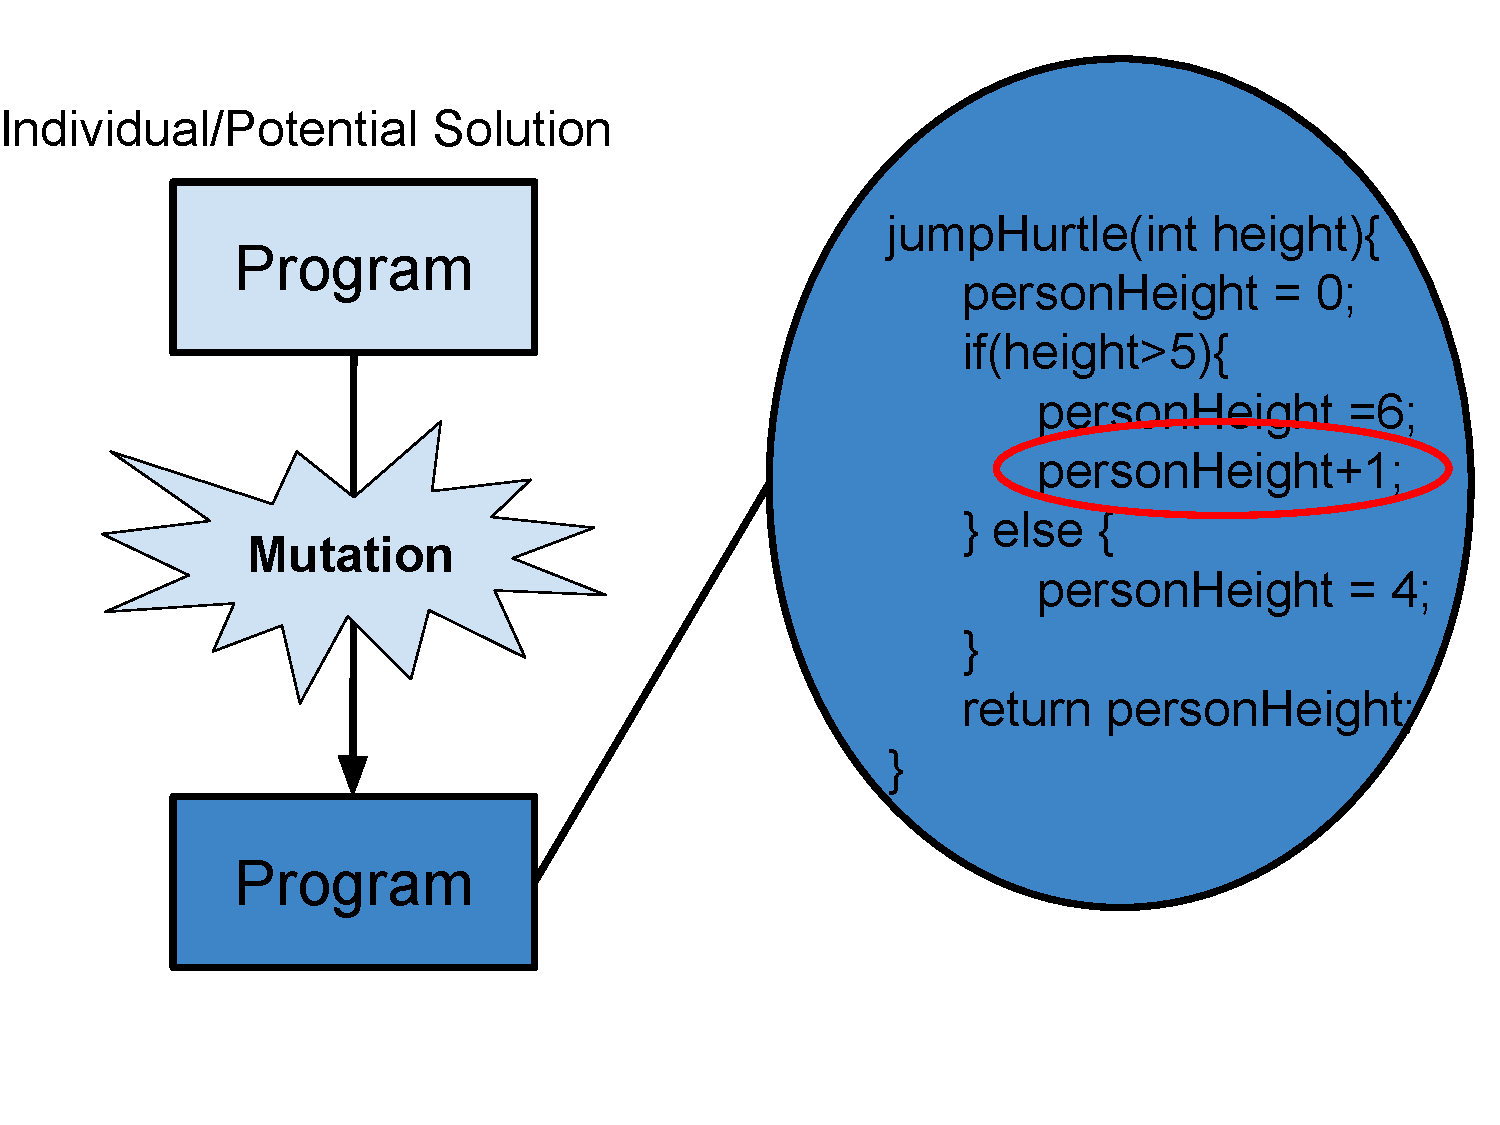
\includegraphics[height=.9\textheight]{Illustrations/gp_5.PDF}
\end{frame}

\section[Hyper-heuristics]{Hyper-heuristics}
\subsection{Heuristics}

\begin{frame}
	\frametitle{Heuristics}
	\begin{columns}
		\begin{column}{.6\textwidth}
			\textbf{Heuristics}~--~a function that ranks alternatives in a search algorithm at each branching step and uses that information to choose which branch to follow.
		\end{column}
		\begin{column}{.4\textwidth}
			\pause
			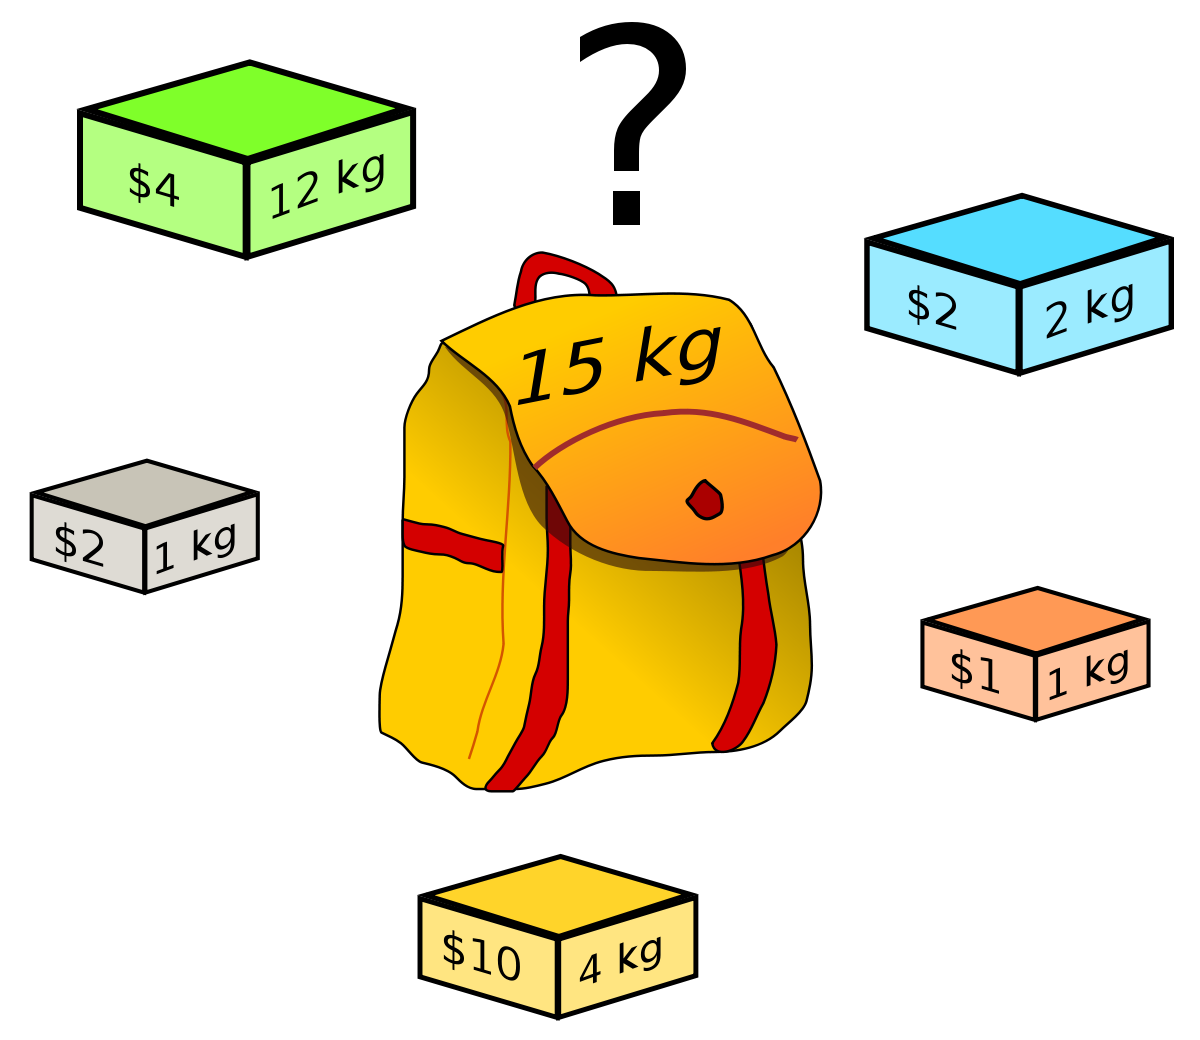
\includegraphics[height=.45\textheight]{Illustrations/knapsack.PNG}
			\\
			\only{\tiny{\url{https://upload.wikimedia.org/wikipedia/commons/thumb/f/fd/Knapsack.svg/1200px-Knapsack.svg.png} }}
		\end{column}
	\end{columns}
\end{frame}

\subsection{Metaheuristics}

\begin{frame}
	\frametitle{Metaheuristic}
	\textbf{Metaheuristic}~--~a heuristic that does not require knowledge about the problem and is not problem specific
	\linespace
\end{frame}

\subsection{Hyper-heuristics}

\begin{frame}
	\frametitle{Heuristics and Metaheuristics}
	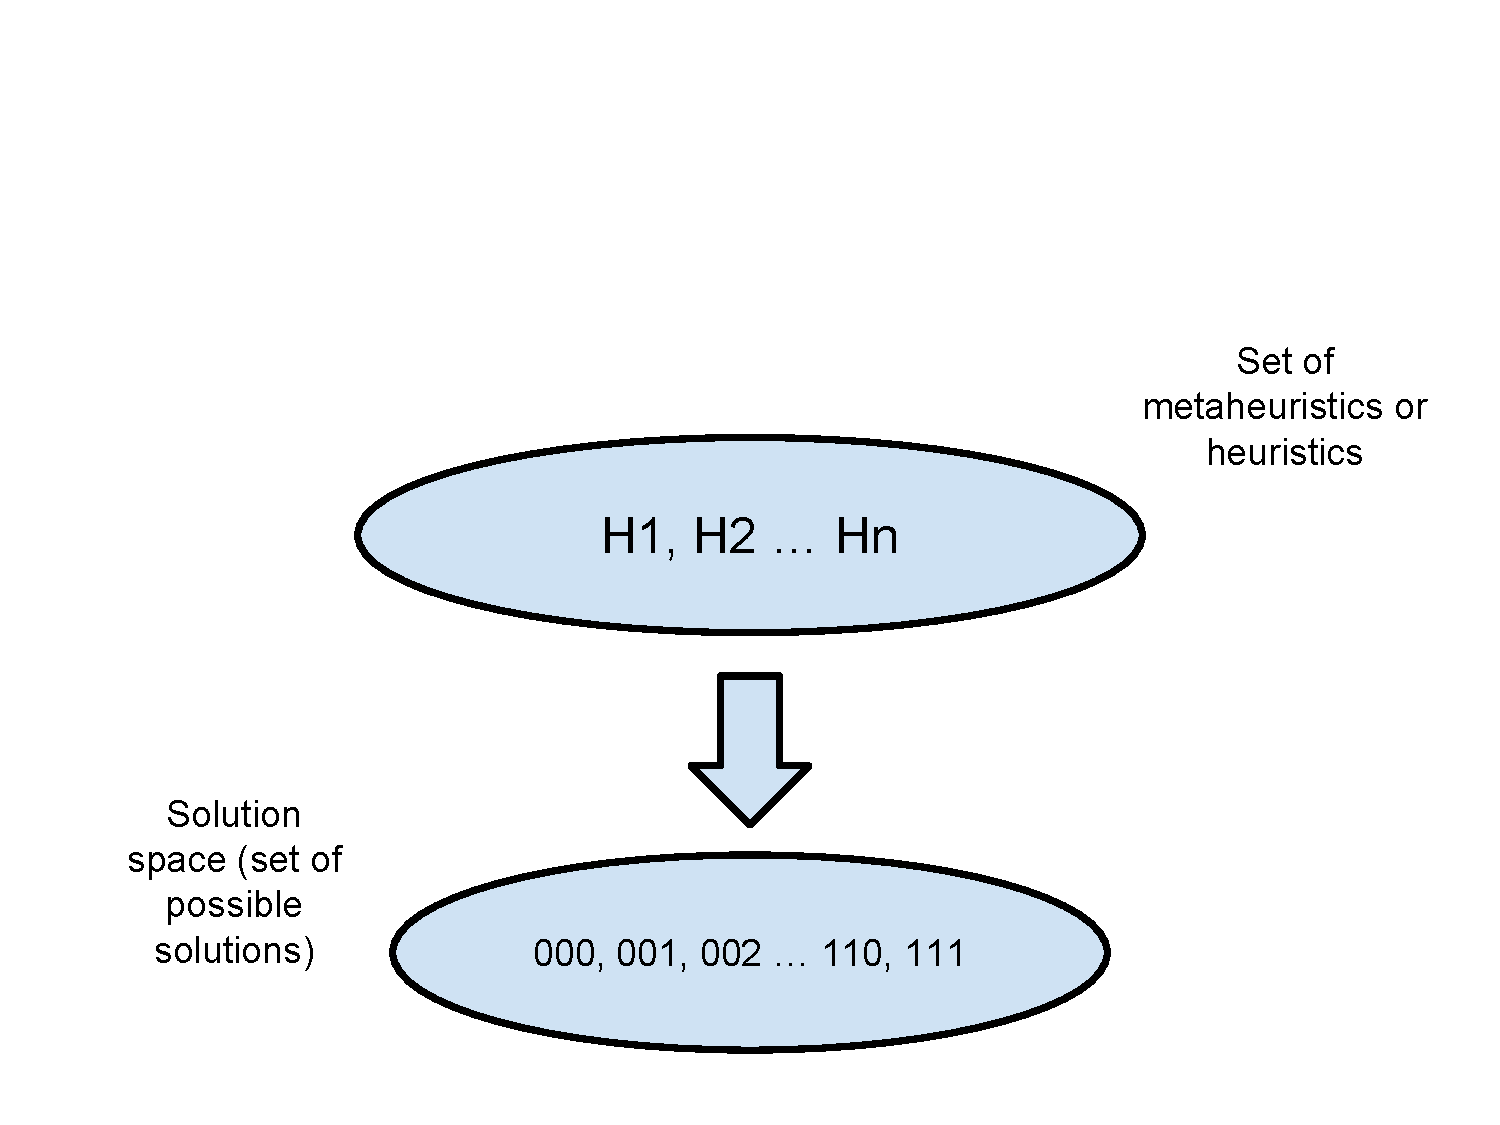
\includegraphics[height=.9\textheight]{Illustrations/heuristic_1.PDF}
\end{frame}

\begin{frame}
	\frametitle{Hyper-heuristics}
	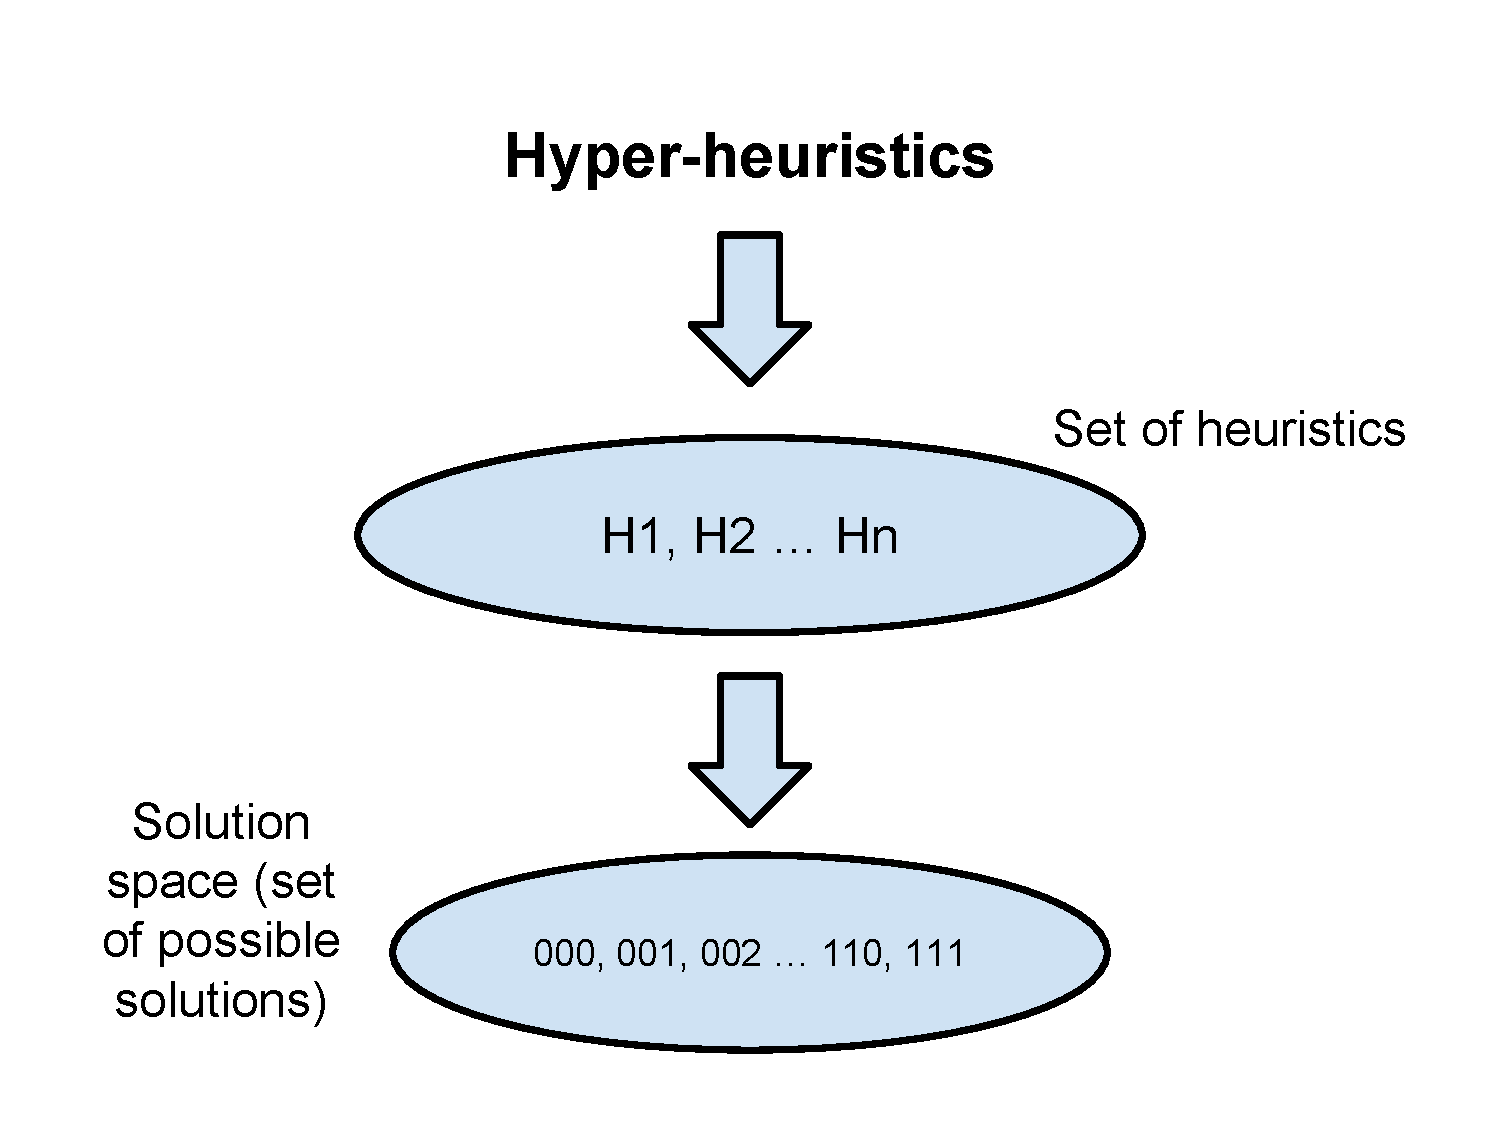
\includegraphics[height=.9\textheight]{Illustrations/heuristic_2.PDF}
\end{frame}

\begin{frame}
	\frametitle{Hyper-heuristics}
	\textbf{Hyper-heuristics}~--~heuristic search methods which seek to automate the process of selecting, generating, or adapting several simpler heuristics in order to solve computational search problems.
	\linespace
	\pause
	\textbf{Genetic programming hyper-heuristics}~--~hyper-heuristics that use genetic programming for the process of selecting, generating, or adapting several simpler heuristics.
\end{frame}

\section[GP Variants]{Genetic Programming Variants}

\subsection{What are they?}

\begin{frame}
	\frametitle{Genetic programming variants}
	\textbf{GP variants}~--~variations on the structure and setup of a genetic programming system.
	\linespace
	\pause
	Harris et al.~\cite{harris:2015} performed an experiment to address whether or not the GP variant used affected the success of the hyper-heuristic
	\linespace
	\pause
	GP variants tested:
	\begin{itemize}
		\item Cartesian GP
		\item Linear GP
		\item Stack-based GP
		\item Tree-based GP
		\item Grammatical Evolution
	\end{itemize}
\end{frame}

\subsection{Why should we care?}
\begin{frame}
	\frametitle{Why should we care?}
	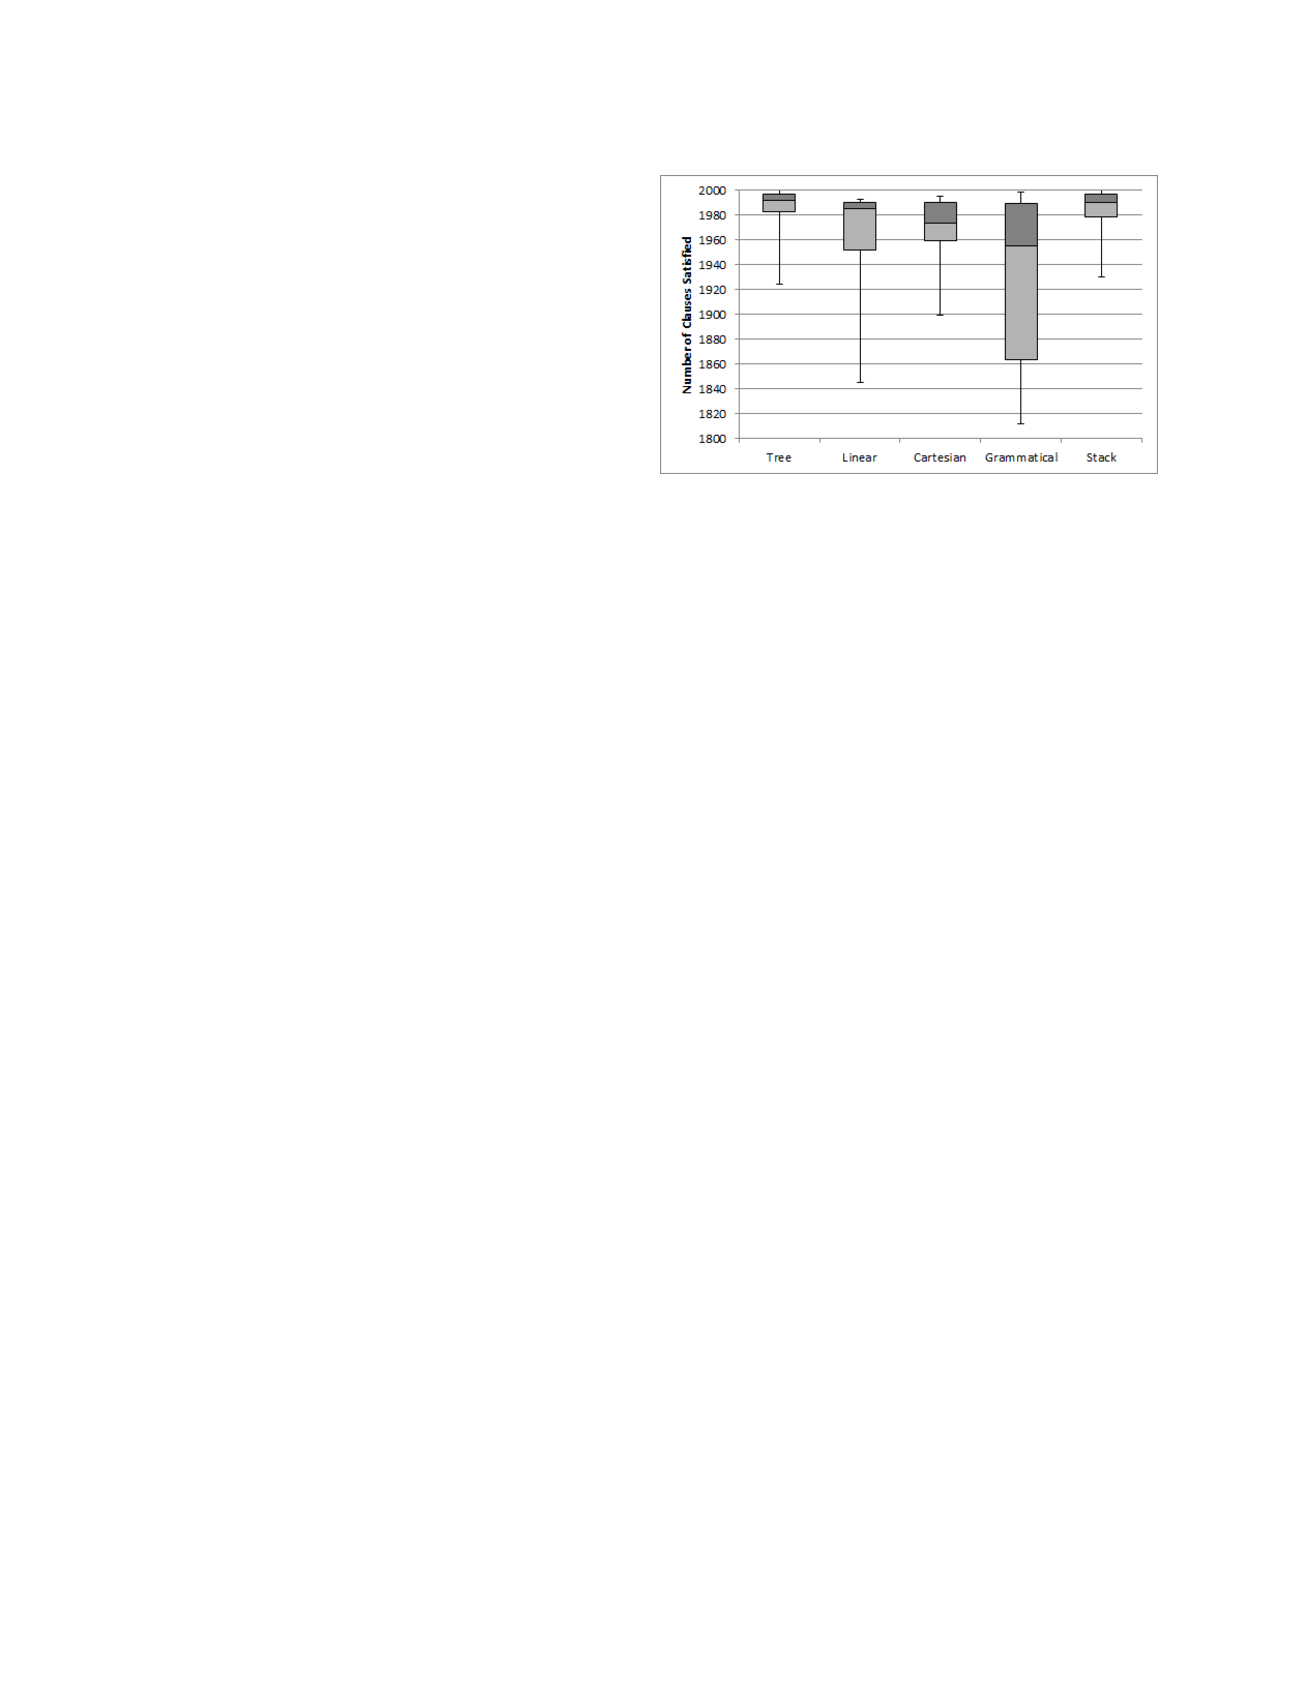
\includegraphics[width=1\textwidth]{Illustrations/gpvariant_graph.PDF}
	\\
\end{frame}

\subsection{Stack-based genetic programming}
\begin{frame}
	\frametitle{Stack-based genetic programming}
	\begin{columns}
		\begin{column}{0.6\textwidth}
			Data-stacks are used for managing input and output of operations.
			\linespace
			\linespace
			\linespace
			\pause Programs are represented as linear sequences of literals and instructions. Below is an example of a simple Push program:
			\[\texttt{(1 2 integer\_equal)}\]
		\end{column}
	\begin{column}{0.4\textwidth}
		\pause[0] 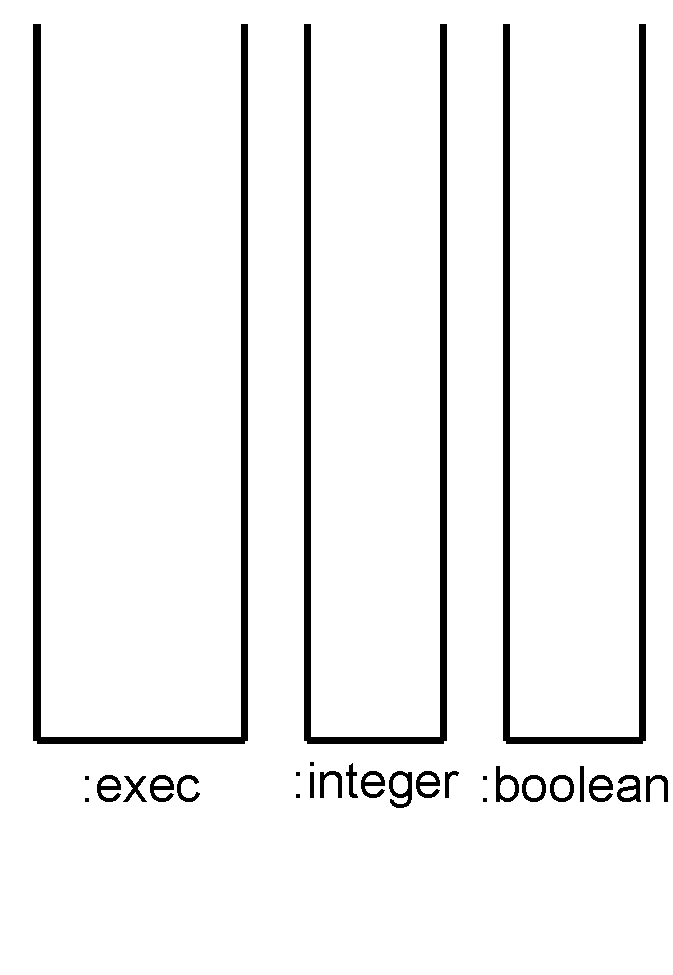
\includegraphics[height=1.2\textwidth]{Illustrations/empty_stacks.PDF}
	\end{column}
	\end{columns}
\end{frame}

\begin{frame}
	\frametitle{Stack-based genetic programming}
	\begin{columns}
		\begin{column}{0.6\textwidth}
			Data-stacks are used for managing input and output of operations.
			\linespace
			\linespace
			\linespace
			Programs are represented as linear sequences of literals and instructions. Below is an example of a simple Push program:
			\[\texttt{(1 2 integer\_equal)}\]
		\end{column}
		\begin{column}{0.4\textwidth}
			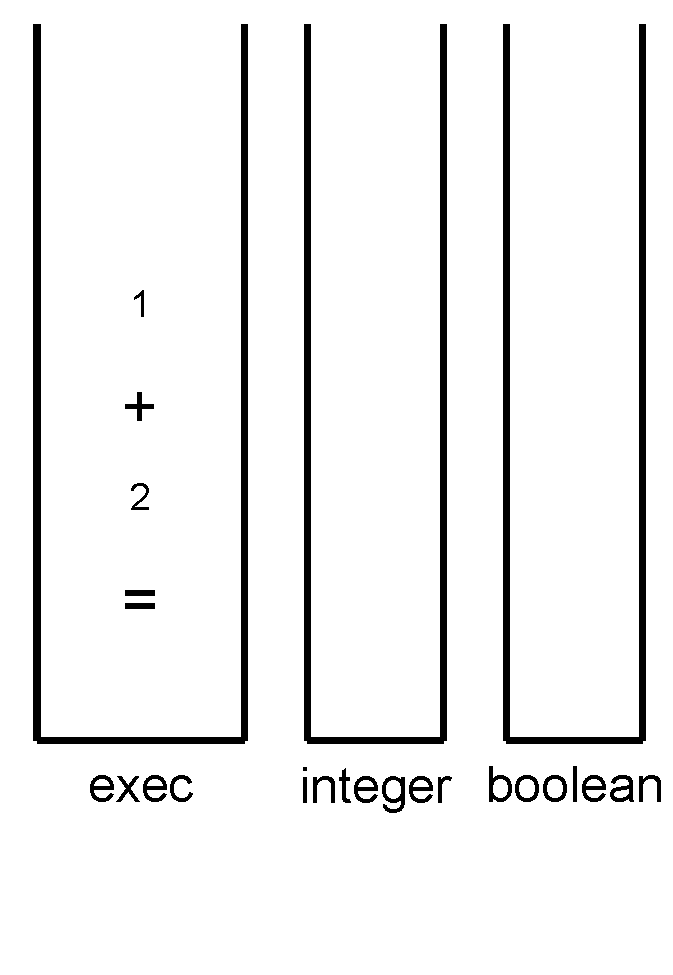
\includegraphics[height=1.2\textwidth]{Illustrations/stack_1.PDF}
		\end{column}
	\end{columns}
\end{frame}

\begin{frame}
	\frametitle{Stack-based genetic programming}
	\begin{columns}
		\begin{column}{0.6\textwidth}
			Data-stacks are used for managing input and output of operations.
			\linespace
			\linespace
			\linespace
			Programs are represented as linear sequences of literals and instructions. Below is an example of a simple Push program:
			\[\texttt{(1 2 integer\_equal)}\]
		\end{column}
		\begin{column}{0.4\textwidth}
			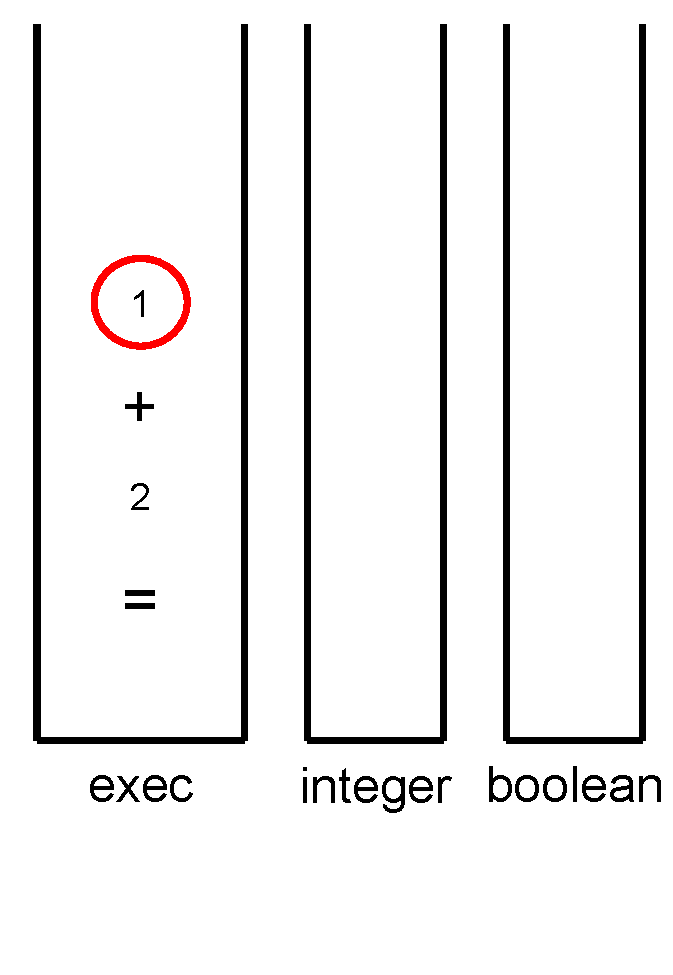
\includegraphics[height=1.2\textwidth]{Illustrations/stack_2.PDF}
		\end{column}
	\end{columns}
\end{frame}

\begin{frame}
	\frametitle{Stack-based genetic programming}
	\begin{columns}
		\begin{column}{0.6\textwidth}
			Data-stacks are used for managing input and output of operations.
			\linespace
			\linespace
			\linespace
			Programs are represented as linear sequences of literals and instructions. Below is an example of a simple Push program:
			\[\texttt{(1 2 integer\_equal)}\]
		\end{column}
		\begin{column}{0.4\textwidth}
			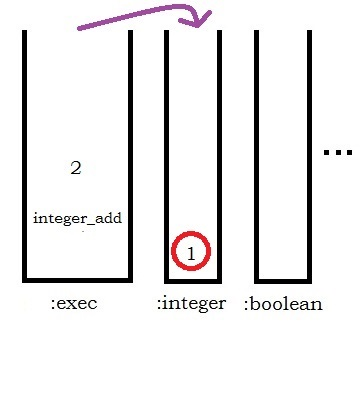
\includegraphics[height=1.2\textwidth]{Illustrations/stack_3.PDF}
		\end{column}
	\end{columns}
\end{frame}

\begin{frame}
	\frametitle{Stack-based genetic programming}
	\begin{columns}
		\begin{column}{0.6\textwidth}
			Data-stacks are used for managing input and output of operations.
			\linespace
			\linespace
			\linespace
			Programs are represented as linear sequences of literals and instructions. Below is an example of a simple Push program:
			\[\texttt{(1 2 integer\_equal)}\]
		\end{column}
		\begin{column}{0.4\textwidth}
			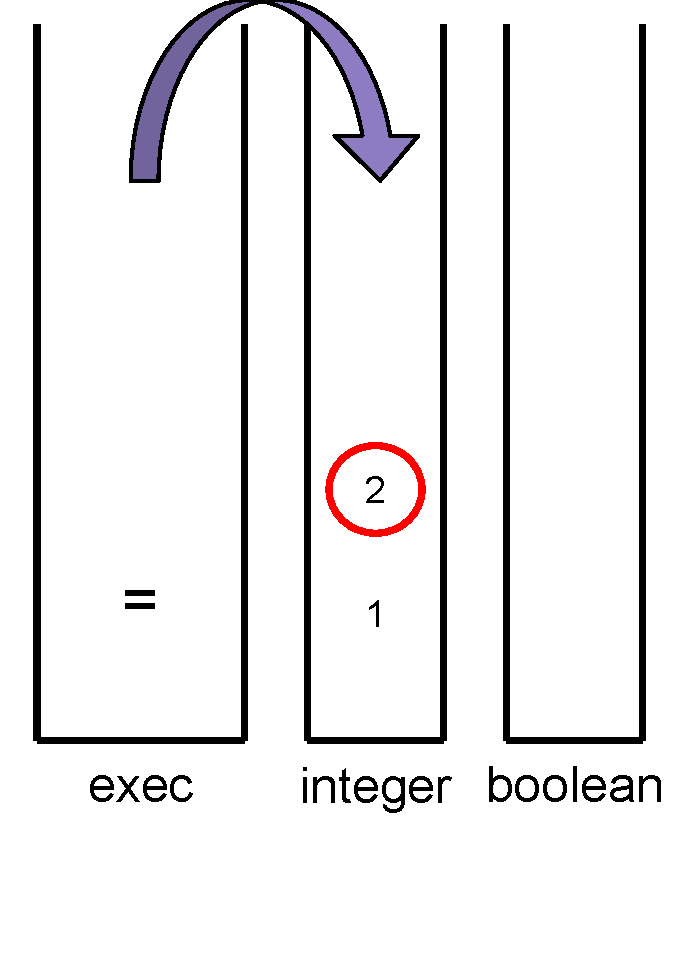
\includegraphics[height=1.2\textwidth]{Illustrations/stack_4.PDF}
		\end{column}
	\end{columns}
\end{frame}

\begin{frame}
	\frametitle{Stack-based genetic programming}
	\begin{columns}
		\begin{column}{0.6\textwidth}
			Data-stacks are used for managing input and output of operations.
			\linespace
			\linespace
			\linespace
			Programs are represented as linear sequences of literals and instructions. Below is an example of a simple Push program:
			\[\texttt{(1 2 integer\_equal)}\]
		\end{column}
		\begin{column}{0.4\textwidth}
			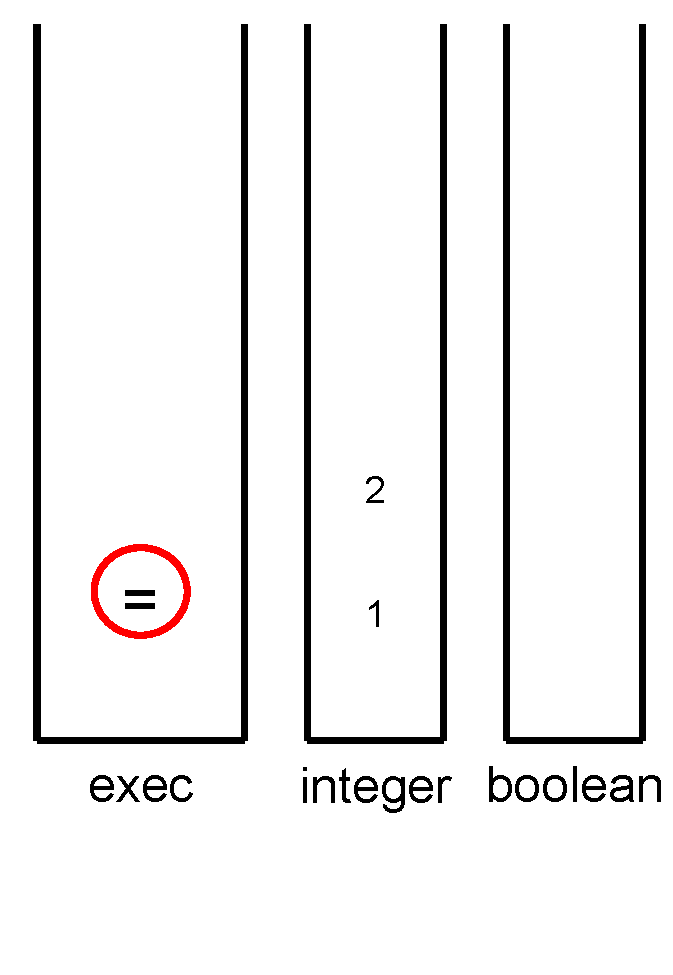
\includegraphics[height=1.2\textwidth]{Illustrations/stack_5.PDF}
		\end{column}
	\end{columns}
\end{frame}

\begin{frame}
	\frametitle{Stack-based genetic programming}
	\begin{columns}
		\begin{column}{0.6\textwidth}
			Data-stacks are used for managing input and output of operations.
			\linespace
			\linespace
			\linespace
			Programs are represented as linear sequences of literals and instructions. Below is an example of a simple Push program:
			\[\texttt{(1 2 integer\_equal)}\]
		\end{column}
		\begin{column}{0.4\textwidth}
			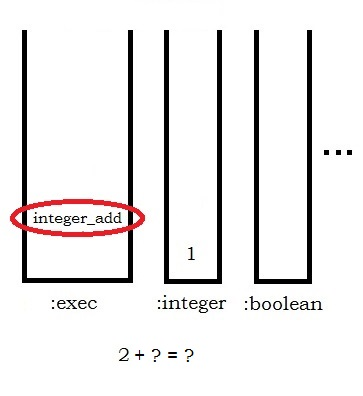
\includegraphics[height=1.2\textwidth]{Illustrations/stack_6.PDF}
		\end{column}
	\end{columns}
\end{frame}

\begin{frame}
	\frametitle{Stack-based genetic programming}
	\begin{columns}
		\begin{column}{0.6\textwidth}
			Data-stacks are used for managing input and output of operations.
			\linespace
			\linespace
			\linespace
			Programs are represented as linear sequences of literals and instructions. Below is an example of a simple Push program:
			\[\texttt{(1 2 integer\_equal)}\]
		\end{column}
		\begin{column}{0.4\textwidth}
			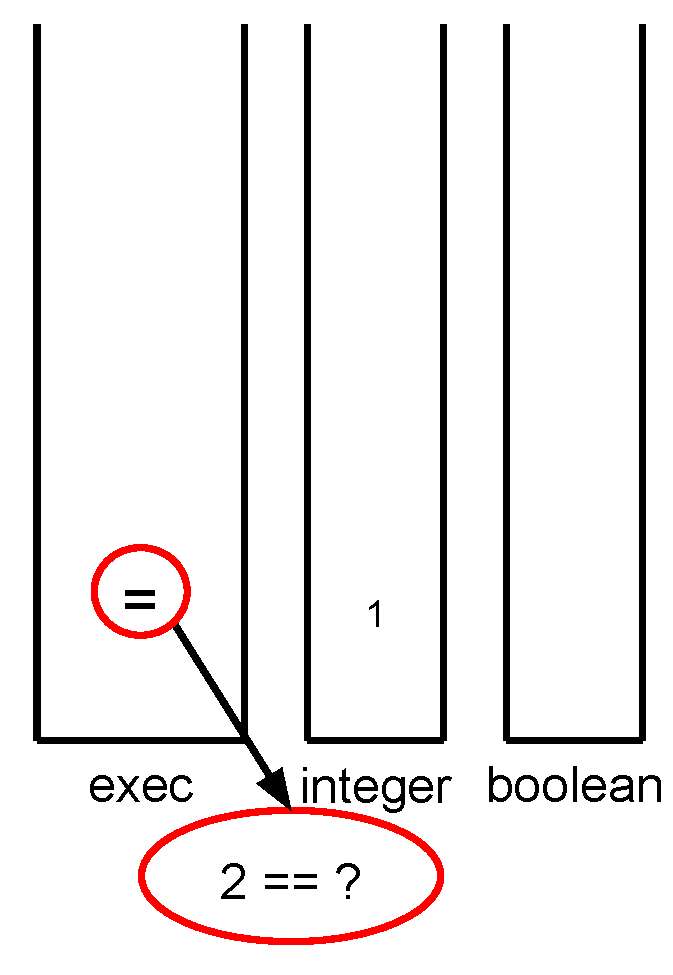
\includegraphics[height=1.2\textwidth]{Illustrations/stack_7.PDF}
		\end{column}
	\end{columns}
\end{frame}

\begin{frame}
	\frametitle{Stack-based genetic programming}
	\begin{columns}
		\begin{column}{0.6\textwidth}
			Data-stacks are used for managing input and output of operations.
			\linespace
			\linespace
			\linespace
			Programs are represented as linear sequences of literals and instructions. Below is an example of a simple Push program:
			\[\texttt{(1 2 integer\_equal)}\]
		\end{column}
		\begin{column}{0.4\textwidth}
			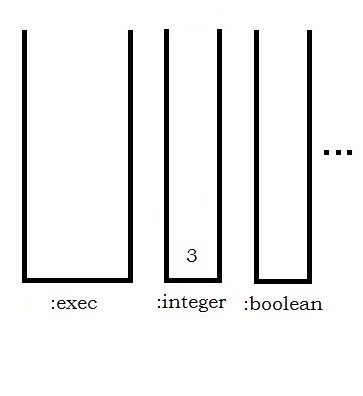
\includegraphics[height=1.2\textwidth]{Illustrations/stack_8.PDF}
		\end{column}
	\end{columns}
\end{frame}

\begin{frame}
	\frametitle{Stack-based genetic programming}
	\begin{columns}
		\begin{column}{0.6\textwidth}
			Data-stacks are used for managing input and output of operations.
			\linespace
			\linespace
			\linespace
			Programs are represented as linear sequences of literals and instructions. Below is an example of a simple Push program:
			\[\texttt{(1 2 integer\_equal)}\]
		\end{column}
		\begin{column}{0.4\textwidth}
			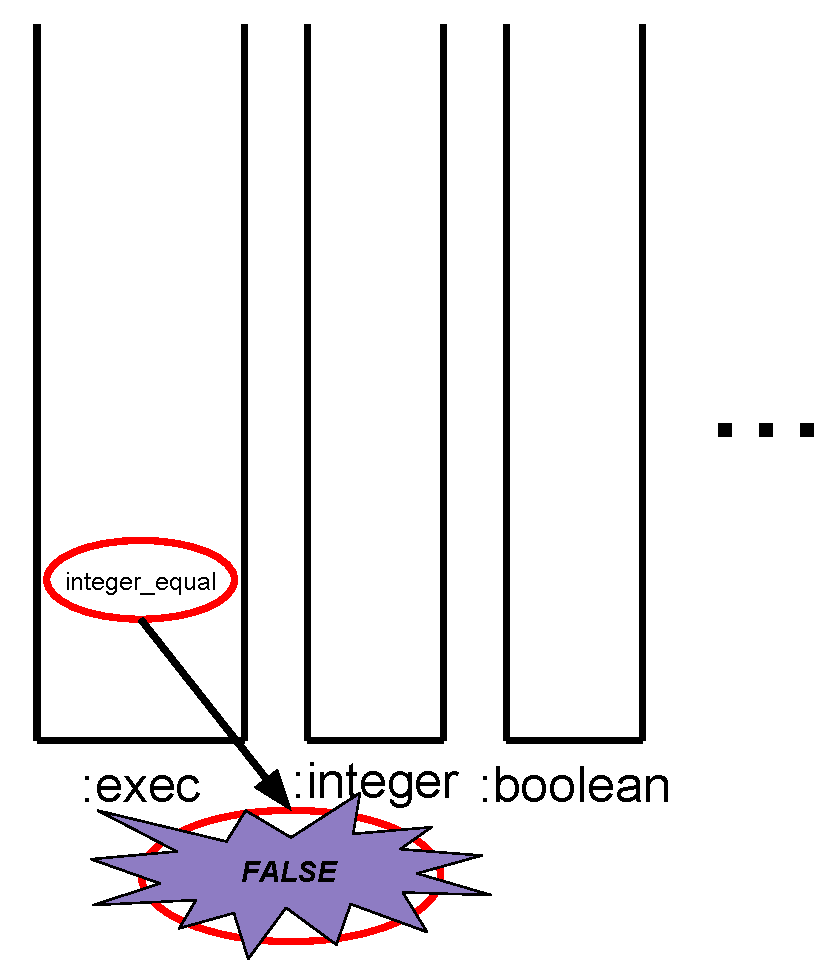
\includegraphics[height=1.2\textwidth]{Illustrations/stack_9.PDF}
		\end{column}
	\end{columns}
\end{frame}

\begin{frame}
	\frametitle{Stack-based genetic programming}
	\begin{columns}
		\begin{column}{0.6\textwidth}
			Data-stacks are used for managing input and output of operations.
			\linespace
			\linespace
			\linespace
			Programs are represented as linear sequences of literals and instructions. Below is an example of a simple Push program:
			\[\texttt{(1 2 integer\_equal)}\]
		\end{column}
		\begin{column}{0.4\textwidth}
			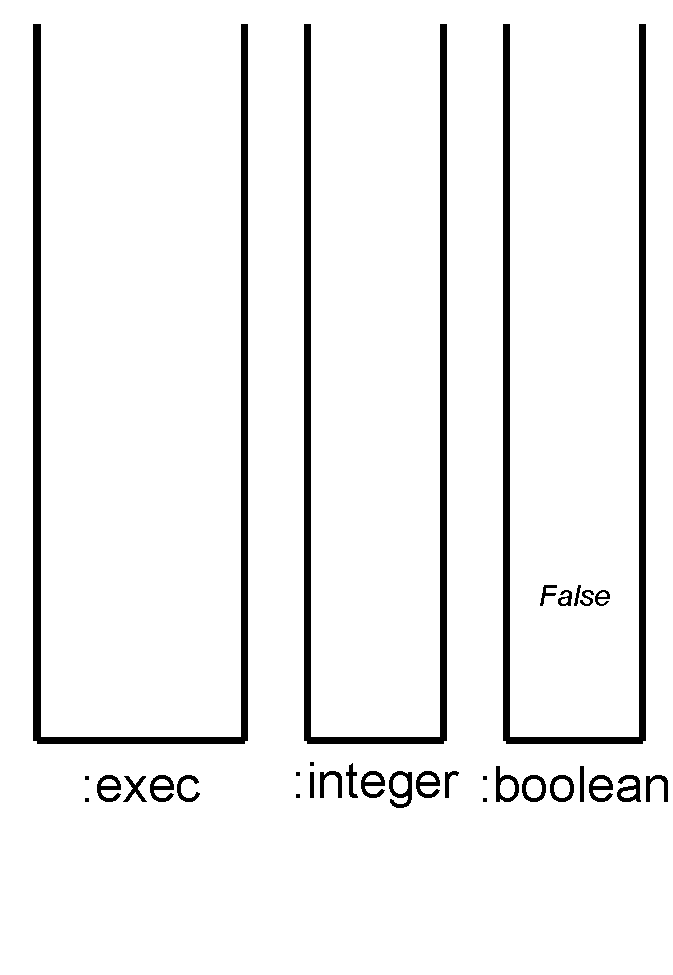
\includegraphics[height=1.2\textwidth]{Illustrations/stack_10.PDF}
		\end{column}
	\end{columns}
\end{frame}

\section[Autoconstruction]{Autoconstruction}

\subsection{What is it?}

\begin{frame}
	\frametitle{What is Autoconstruction?}
	\begin{itemize}
		\item Autoconstruction is a type of genetic programming hyper-heuristic~(GPHH)
		\linespace
		\pause
		\item In most GPHH, the individual programs are evolving, but everything else is specified by the engineer; in autoconstruction, evolution is evolving as well.
		\linespace
		\pause
		\item Programs are responsible for evolving solutions \textit{and} responsible for evolving their offspring.
	\end{itemize}
\end{frame}

\subsection{AutoDoG}

\begin{frame}
	\frametitle{AutoDoG}
	\begin{itemize}
		\item A system designed by Spector et al.~\cite{spector:2016} that uses autoconstruction to evolve programs.
		\linespace
		\pause
		\item Uses the Push programming language
		\linespace
		\pause
		\item Uses Plush, a linear genome format for Push
	\end{itemize}	
\end{frame}

\begin{frame}
	\frametitle{AutoDoG~--~reproduction}
	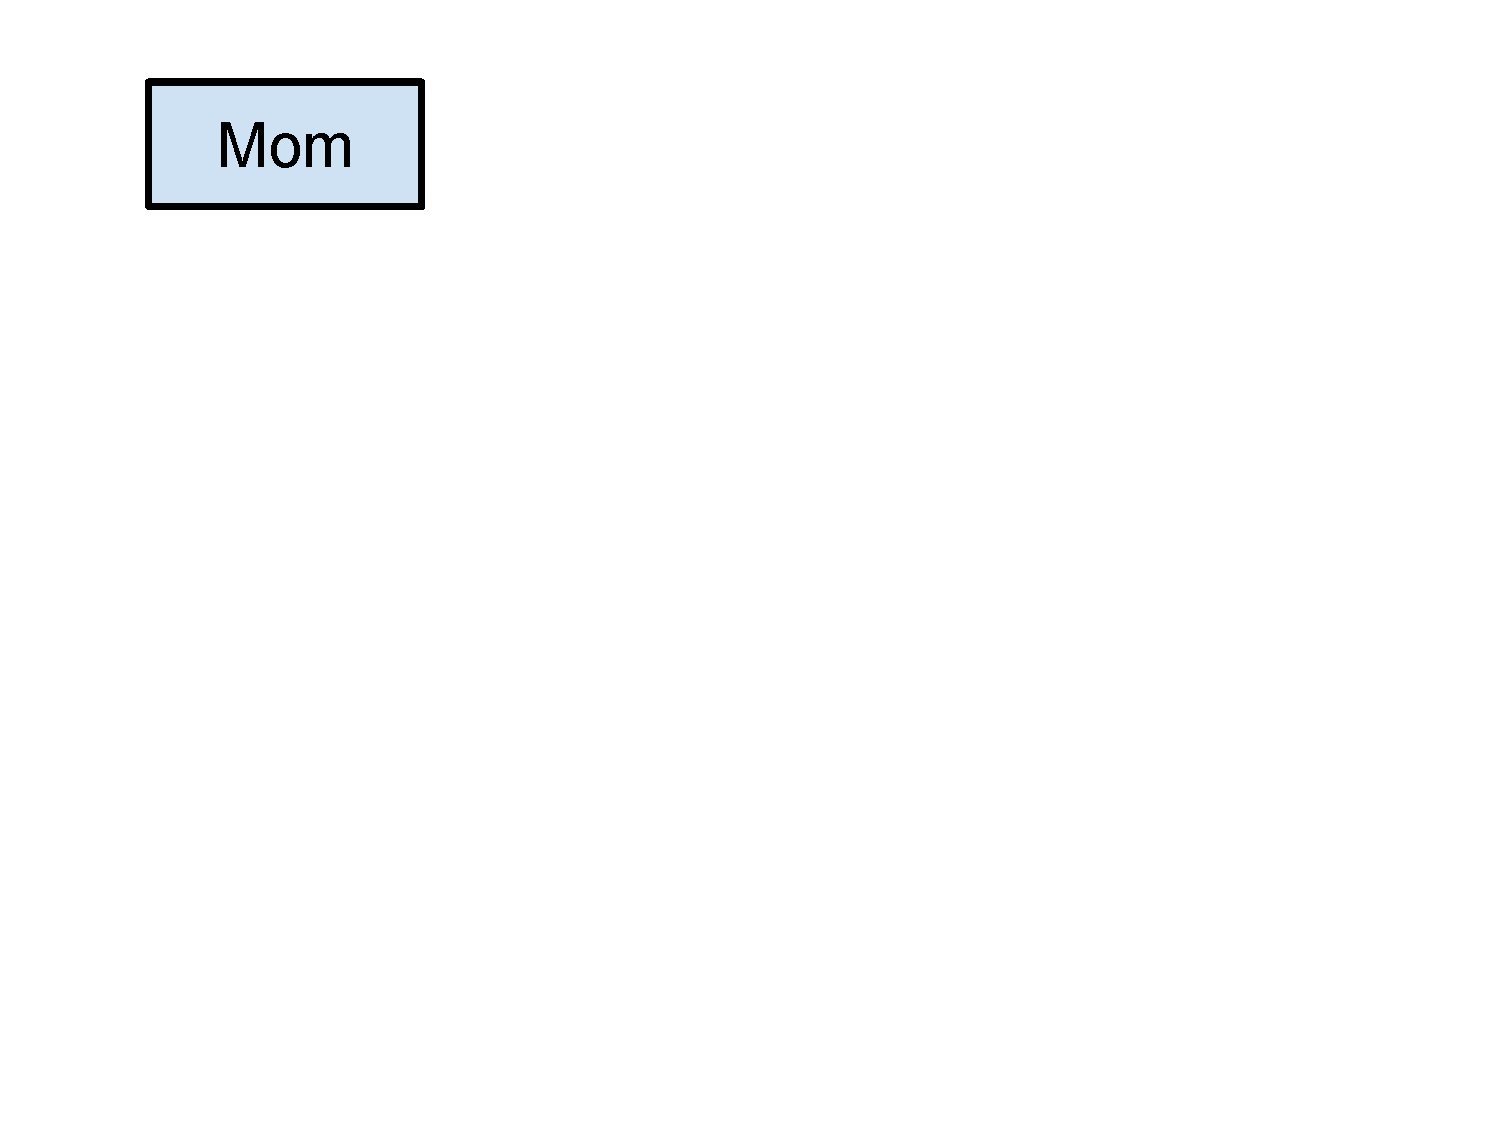
\includegraphics[width=.9\textwidth]{Illustrations/autodog_1.PDF}
\end{frame}

\begin{frame}
	\frametitle{AutoDoG~--~reproduction}
	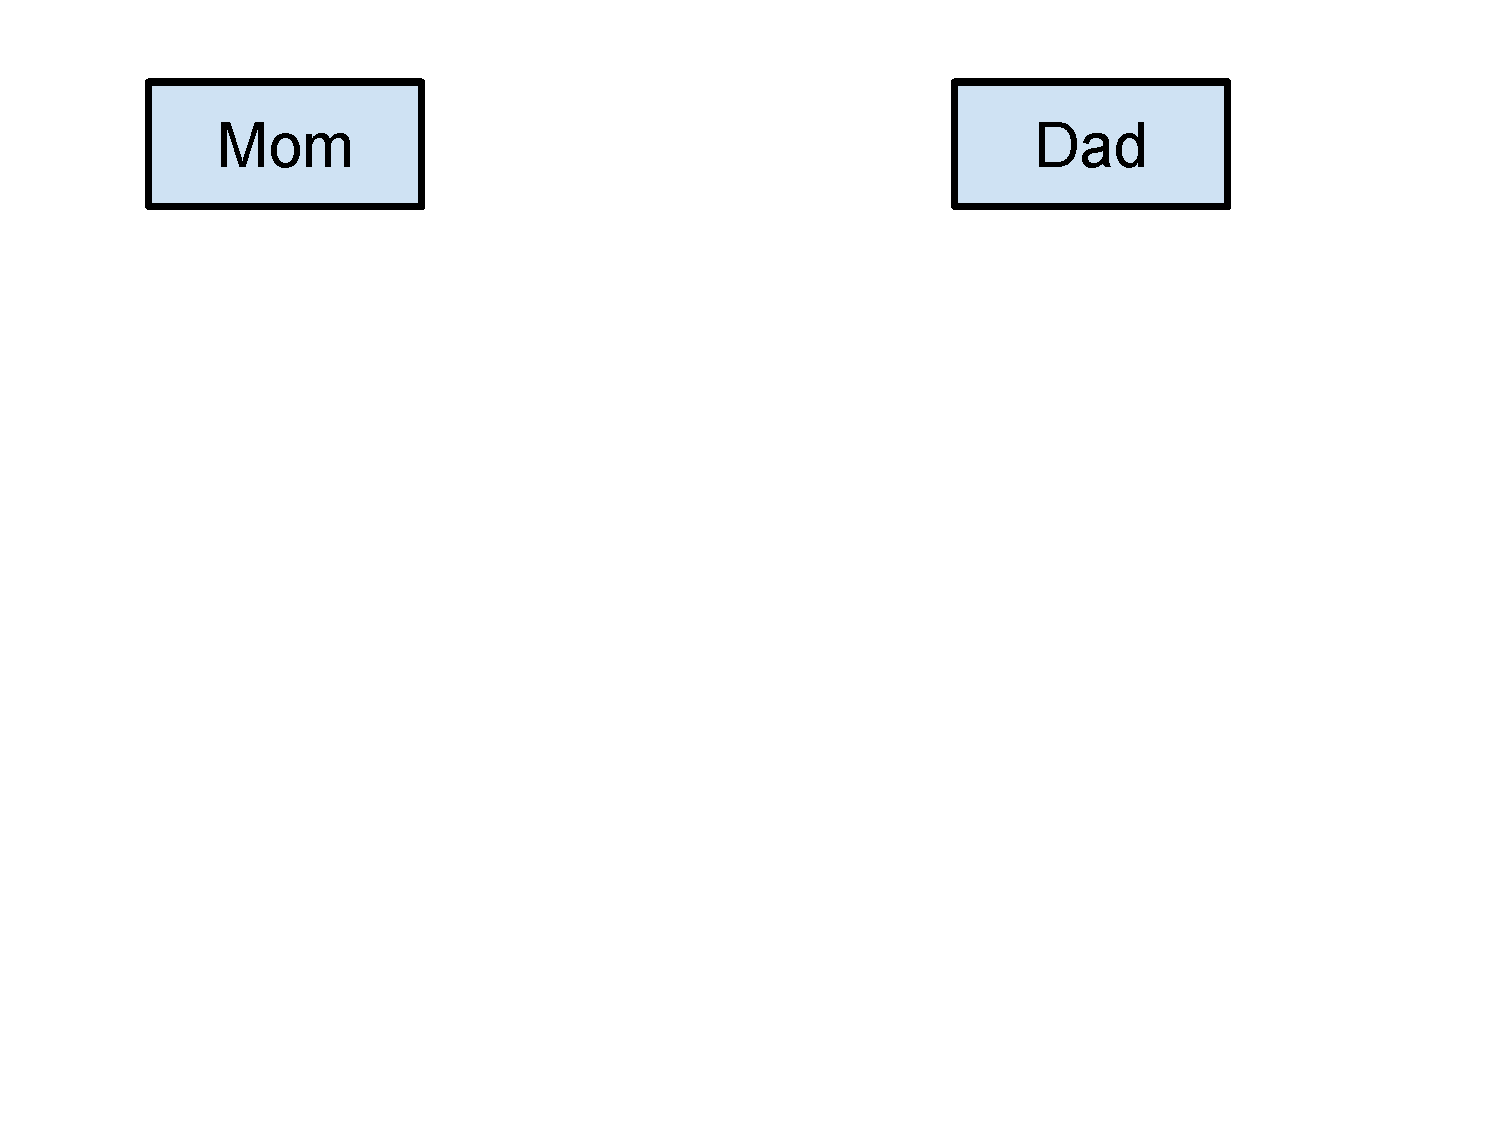
\includegraphics[width=.9\textwidth]{Illustrations/autodog_2.PDF}
\end{frame}

\begin{frame}
	\frametitle{AutoDoG~--~reproduction}
	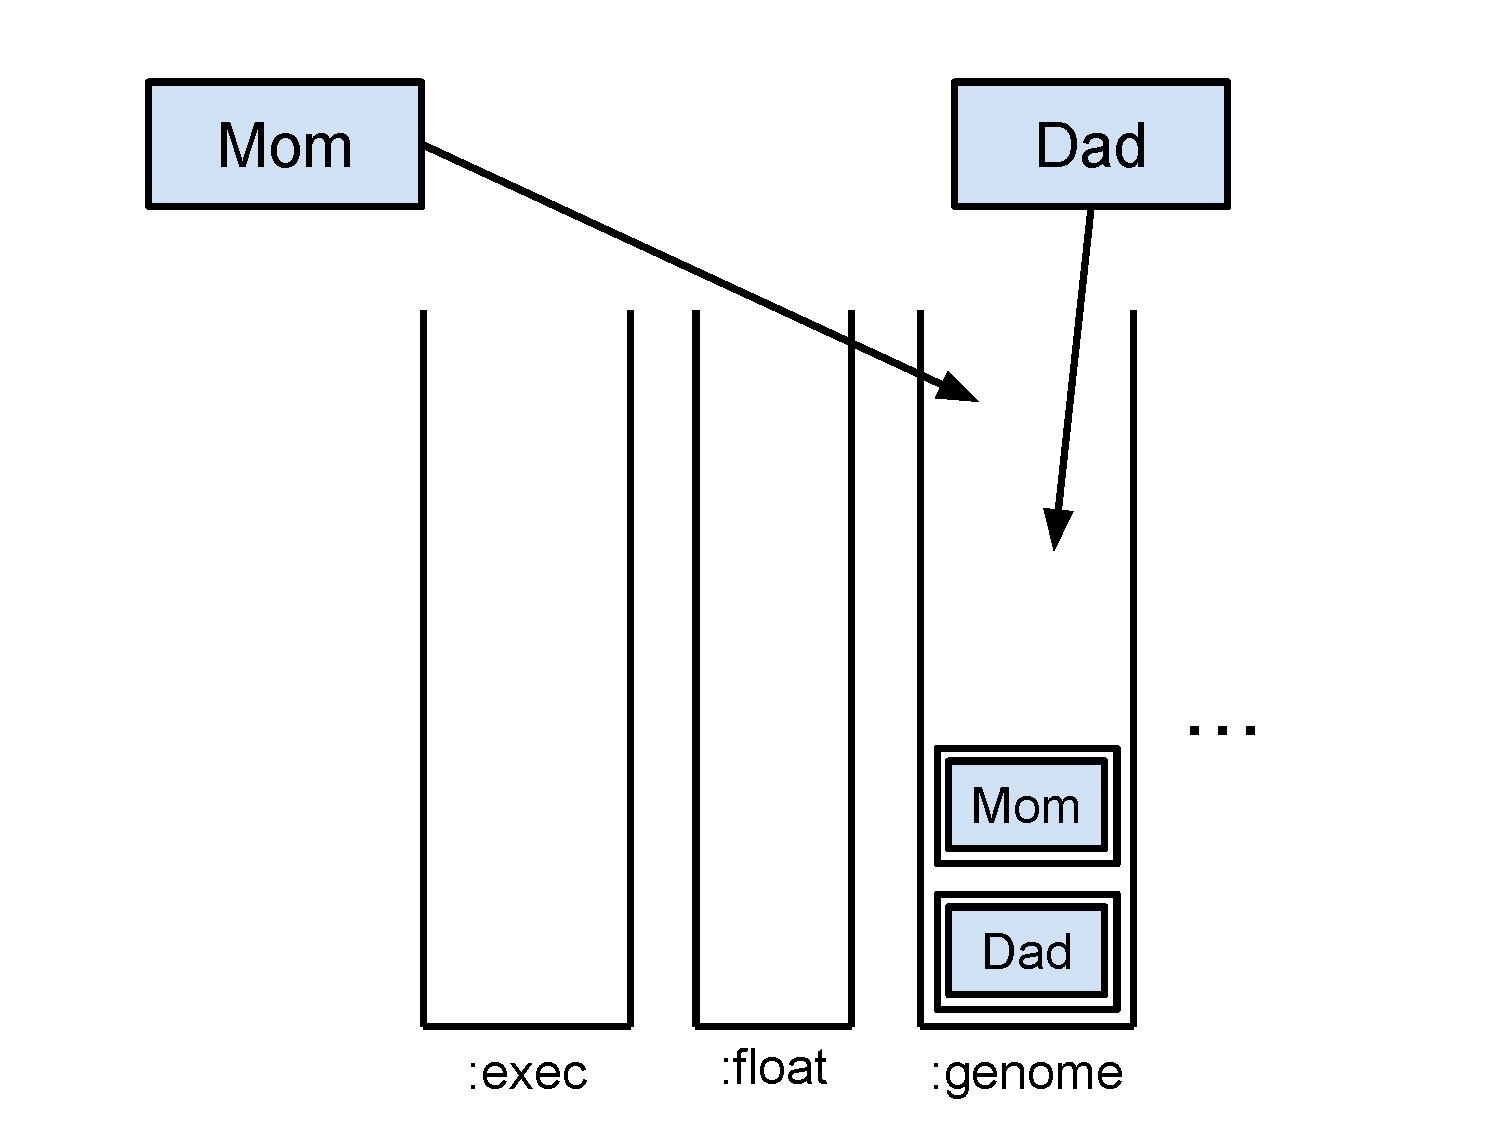
\includegraphics[width=.9\textwidth]{Illustrations/autodog_3.PDF}
\end{frame}

\begin{frame}
	\frametitle{AutoDoG~--~reproduction}
	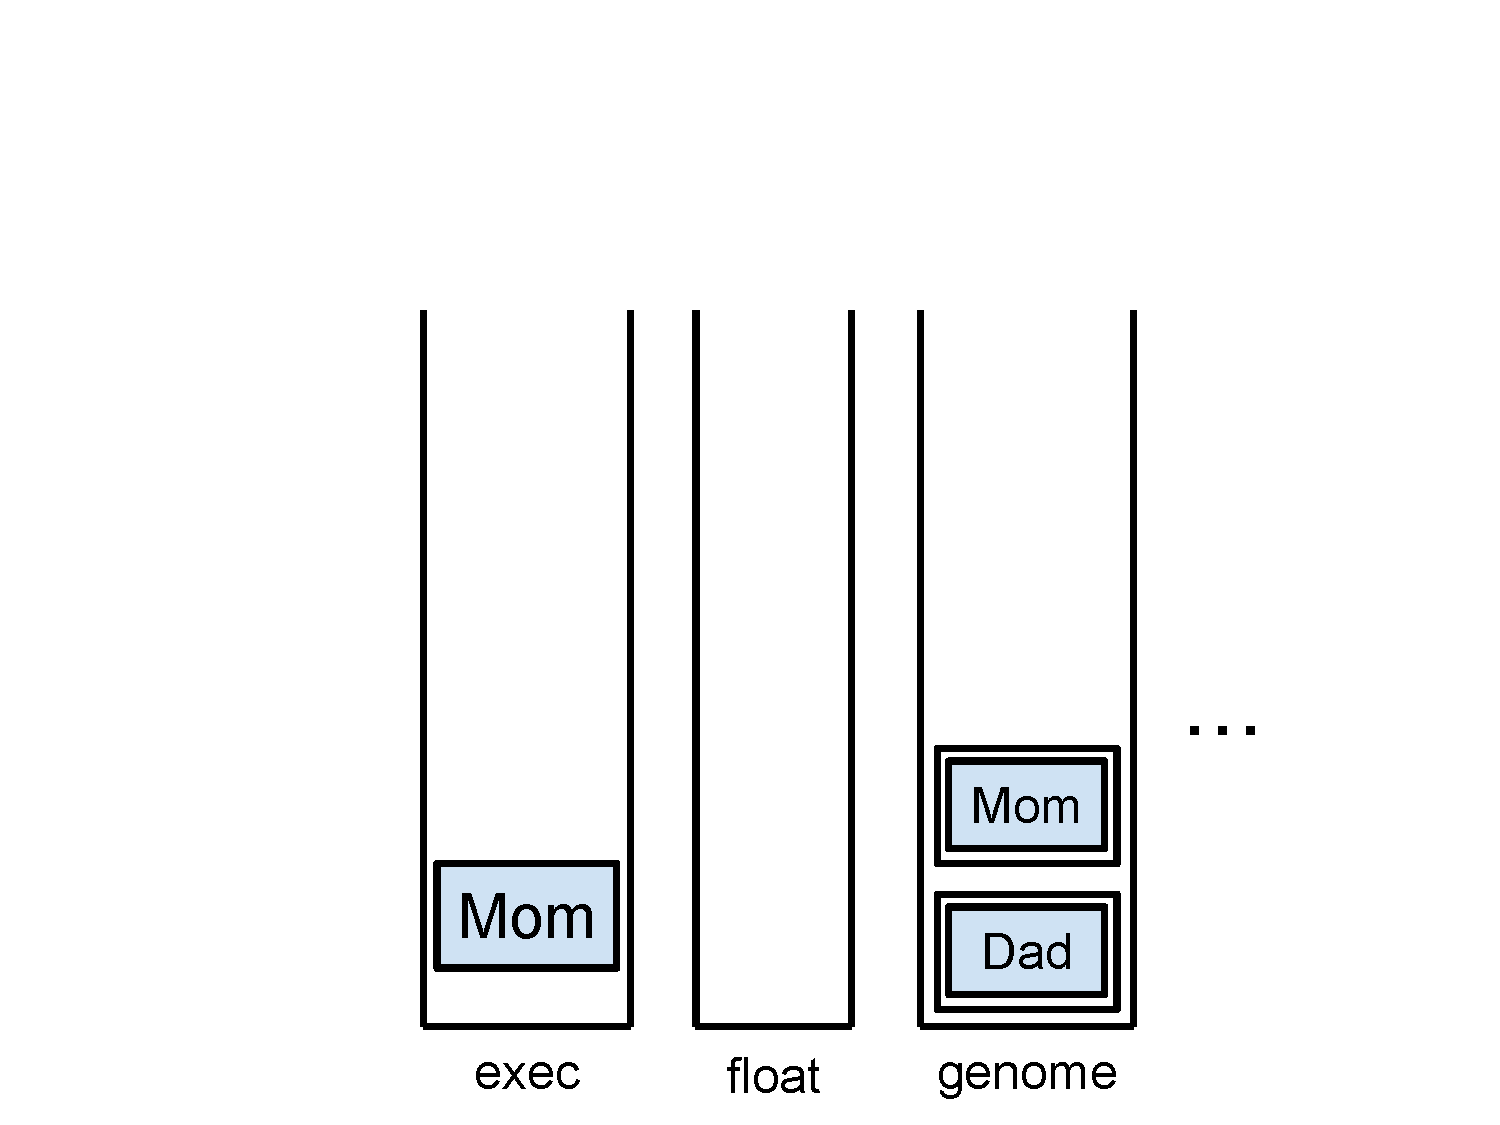
\includegraphics[width=.9\textwidth]{Illustrations/autodog_4.PDF}
\end{frame}

\begin{frame}
	\frametitle{AutoDoG~--~reproduction}
	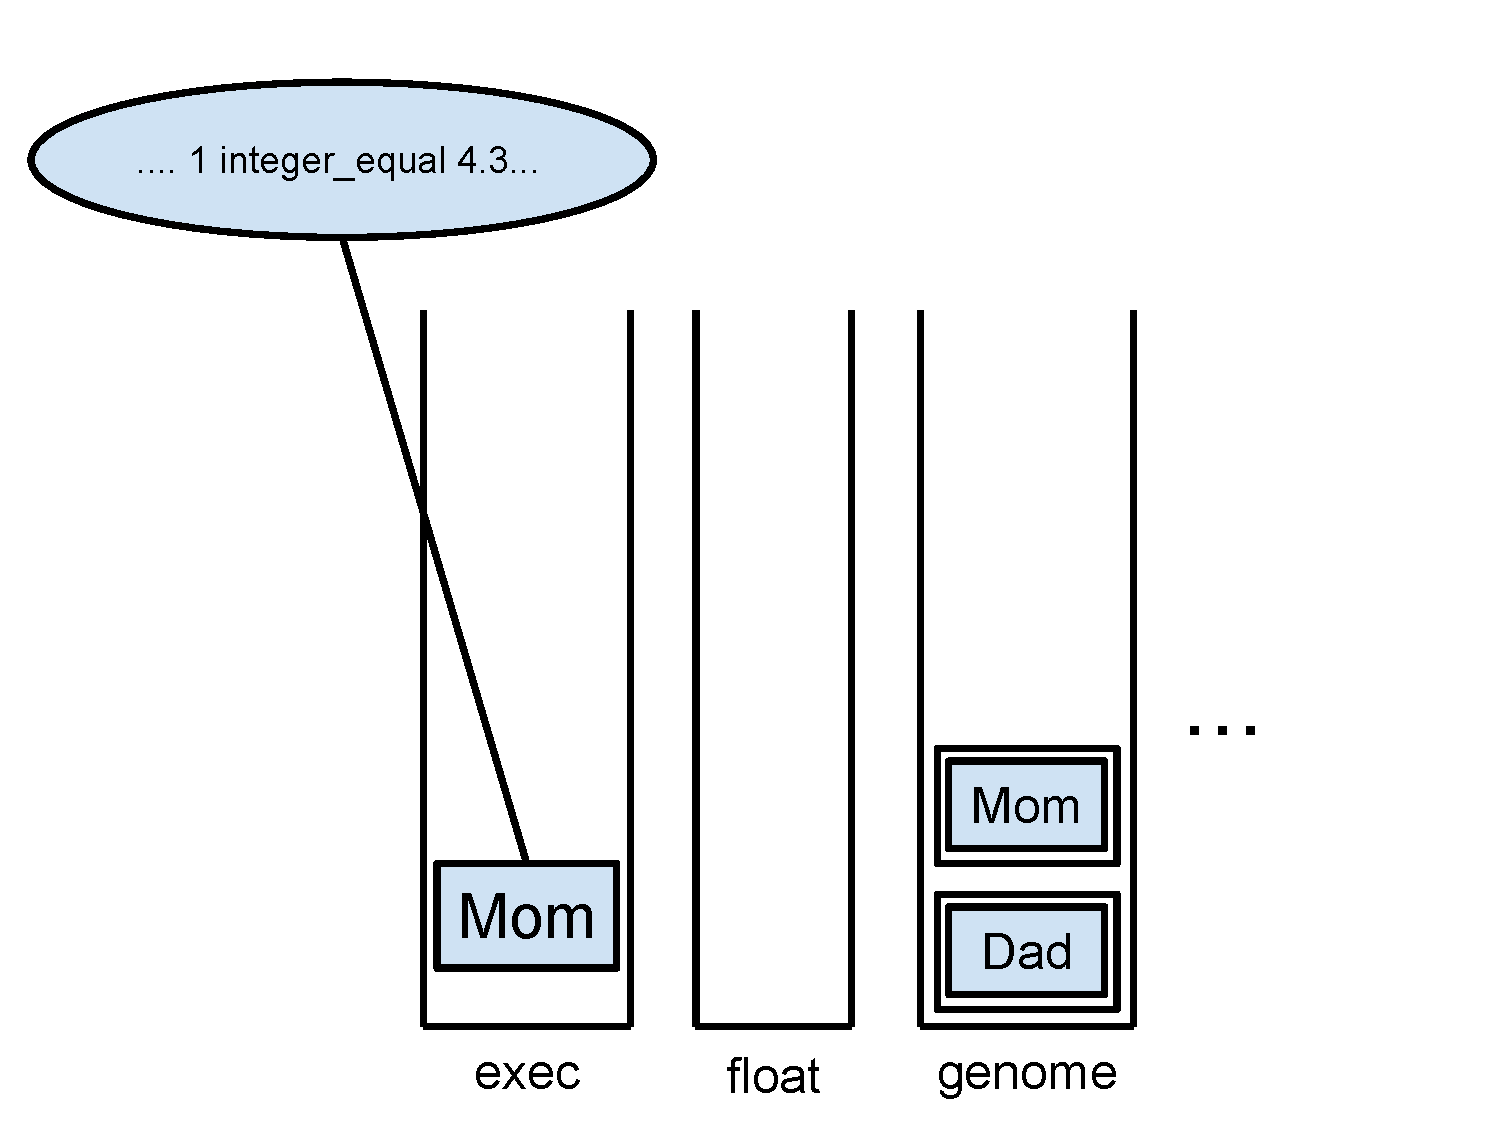
\includegraphics[width=.9\textwidth]{Illustrations/autodog_5.PDF}
\end{frame}

\begin{frame}
	\frametitle{AutoDoG~--~reproduction}
	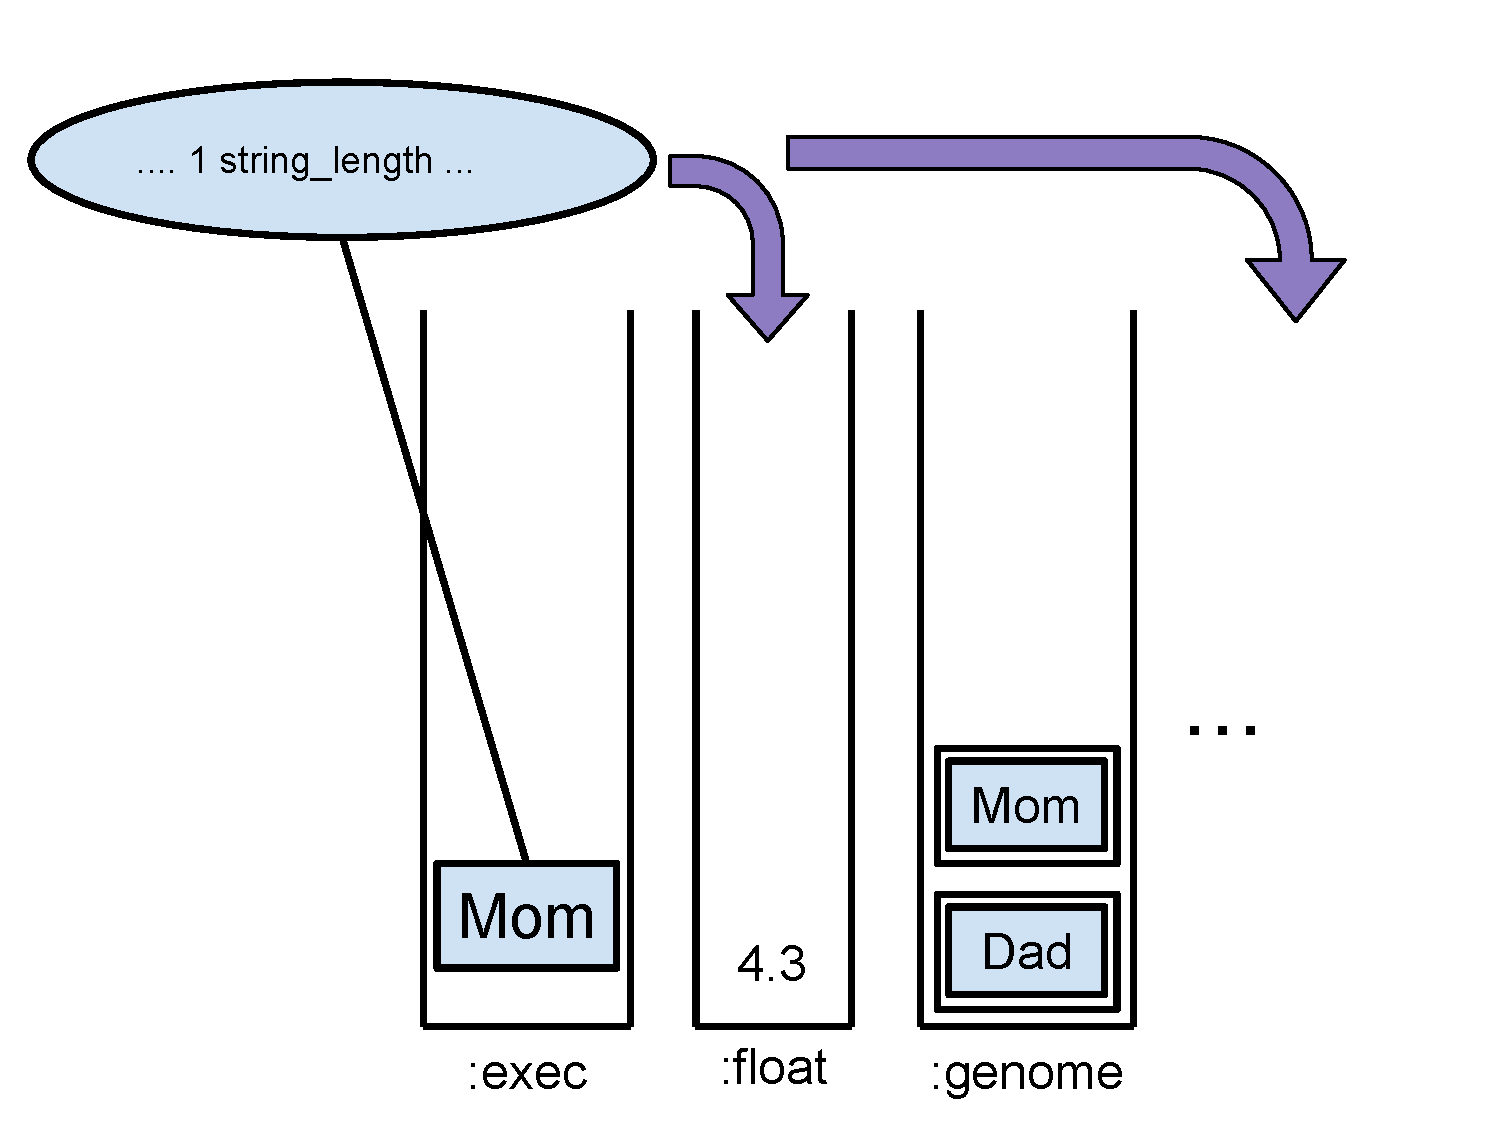
\includegraphics[width=.9\textwidth]{Illustrations/autodog_6.PDF}
\end{frame}

\begin{frame}
	\frametitle{AutoDoG~--~reproduction}
	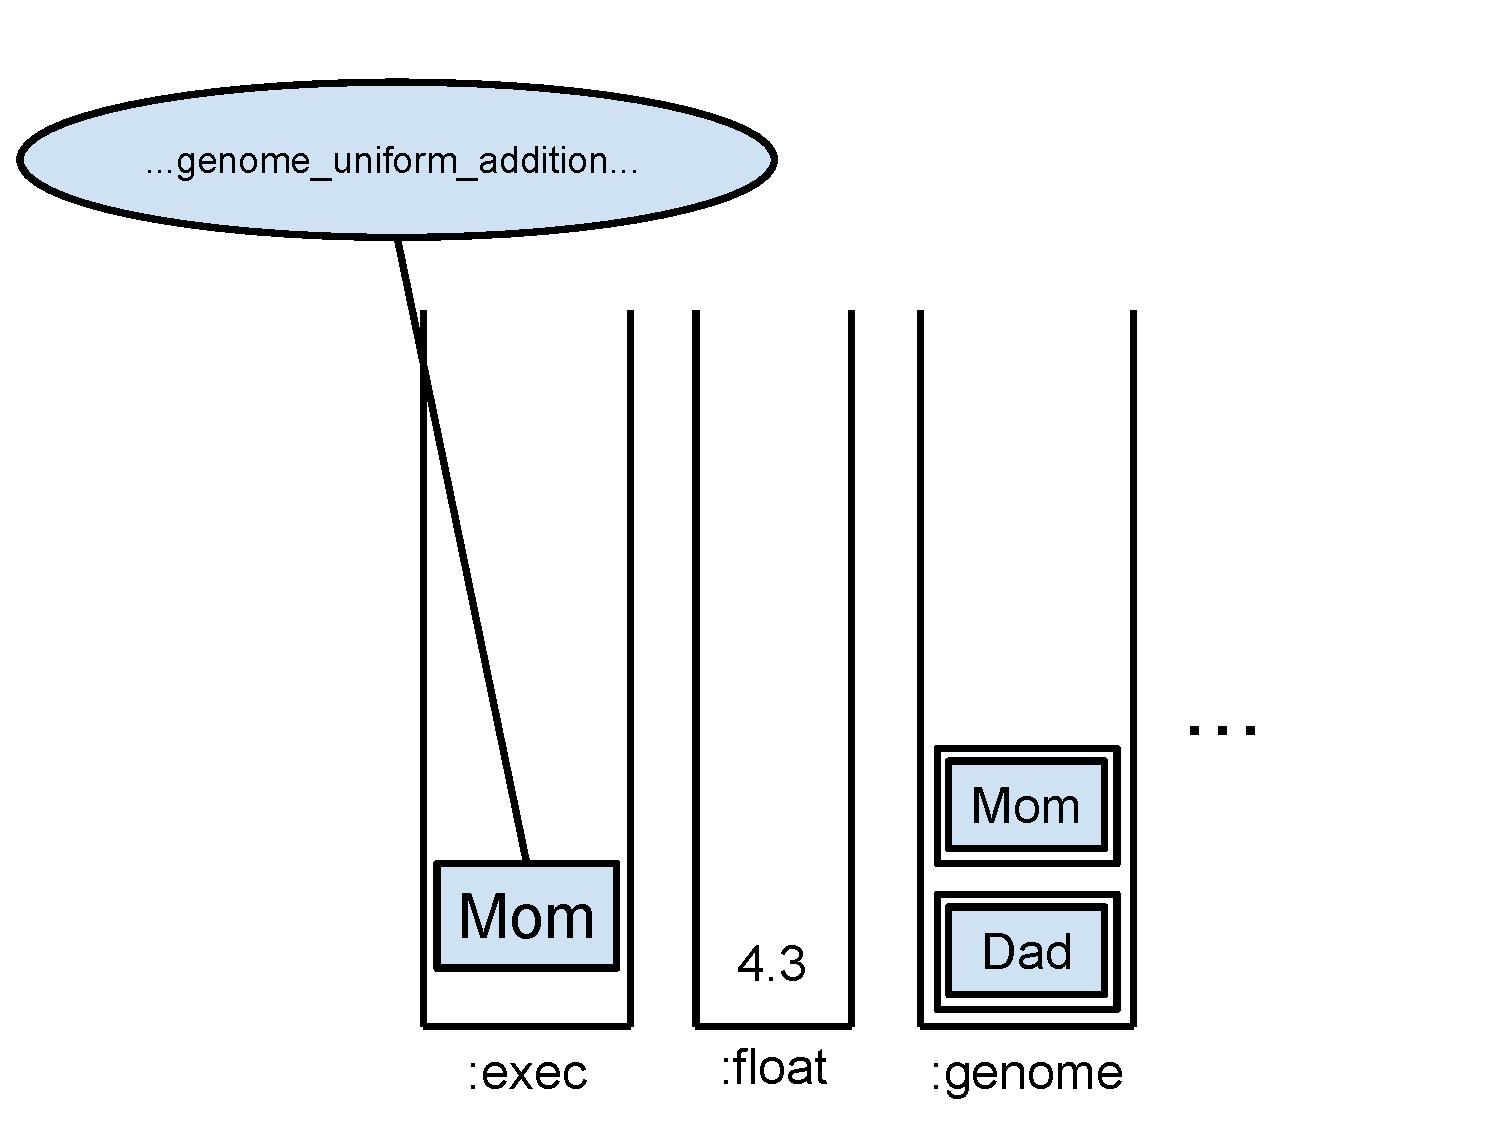
\includegraphics[width=.9\textwidth]{Illustrations/autodog_7.PDF}
\end{frame}

\begin{frame}
	\frametitle{AutoDoG~--~reproduction}
	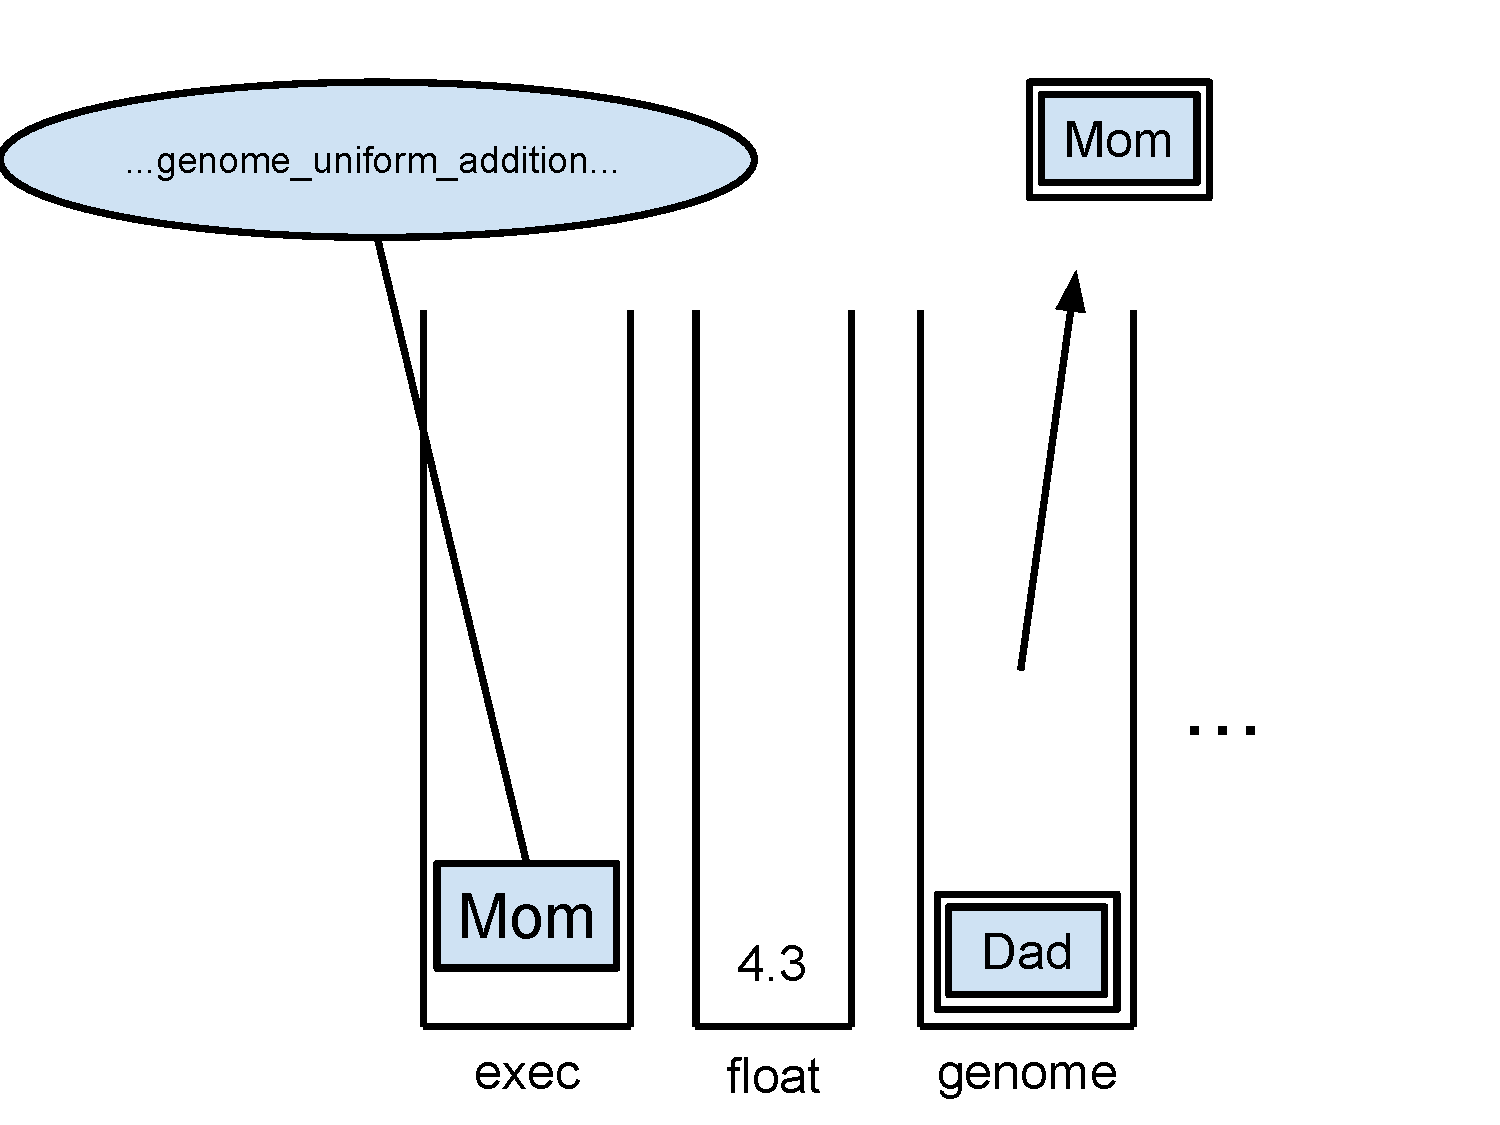
\includegraphics[width=.9\textwidth]{Illustrations/autodog_8.PDF}
\end{frame}

\begin{frame}
	\frametitle{AutoDoG~--~reproduction}
	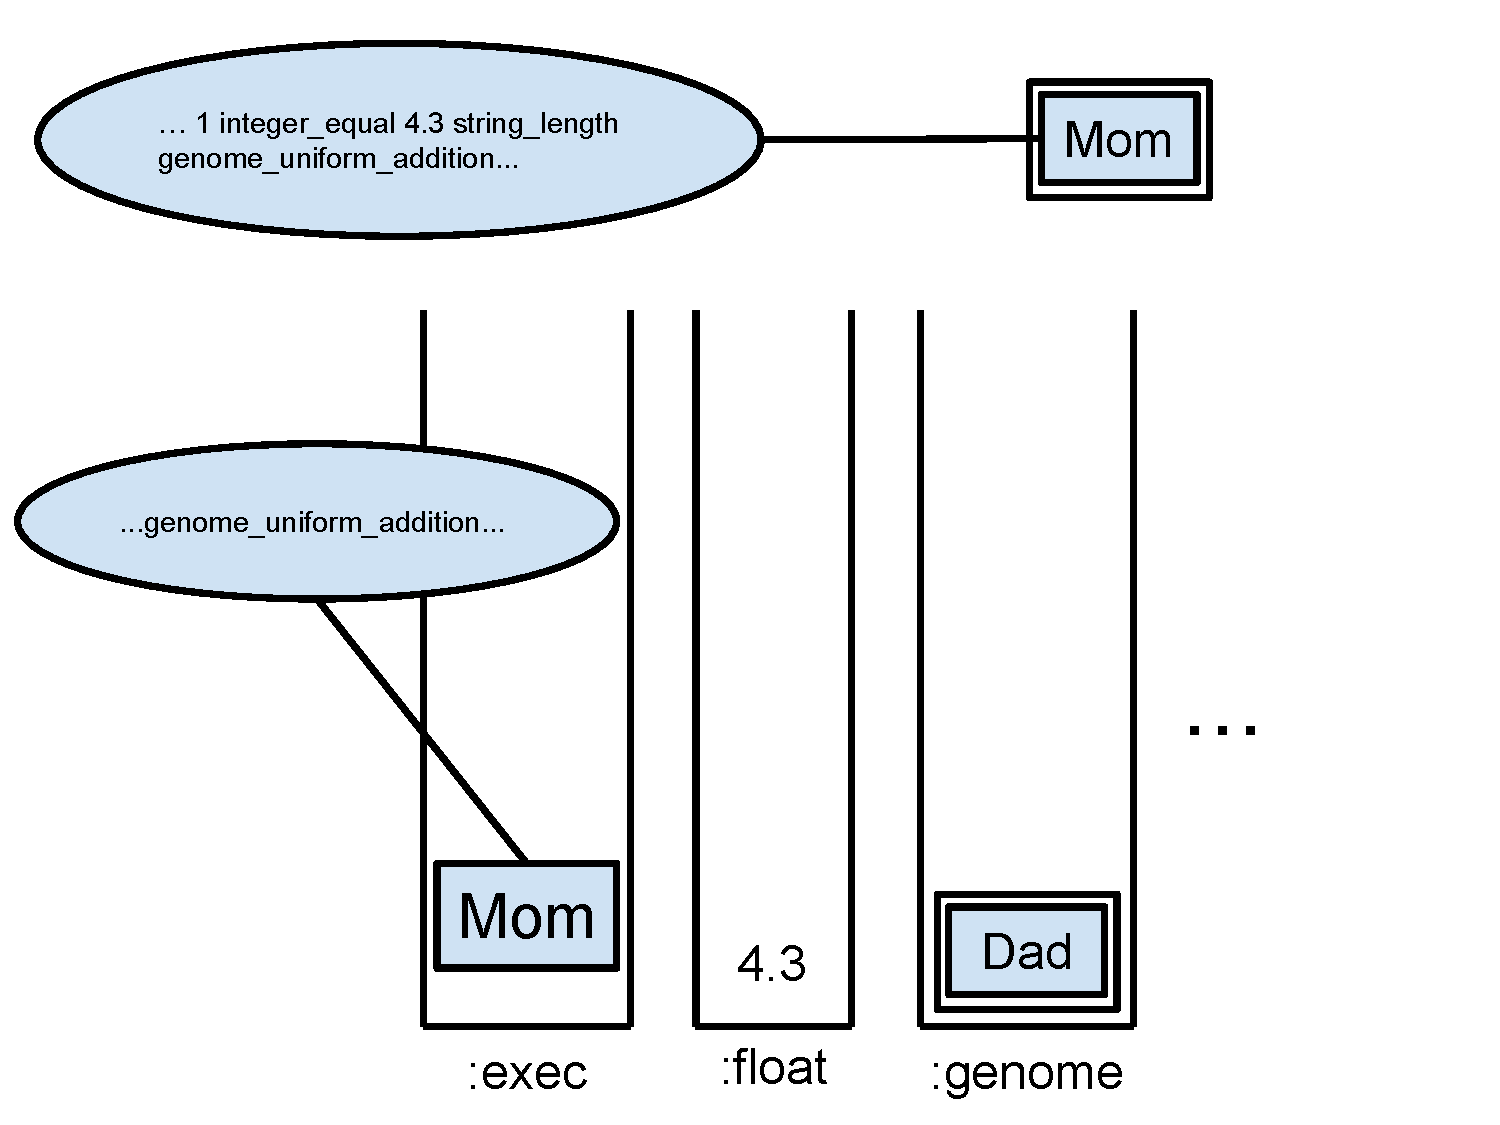
\includegraphics[width=.9\textwidth]{Illustrations/autodog_9.PDF}
\end{frame}

\begin{frame}
	\frametitle{AutoDoG~--~reproduction}
	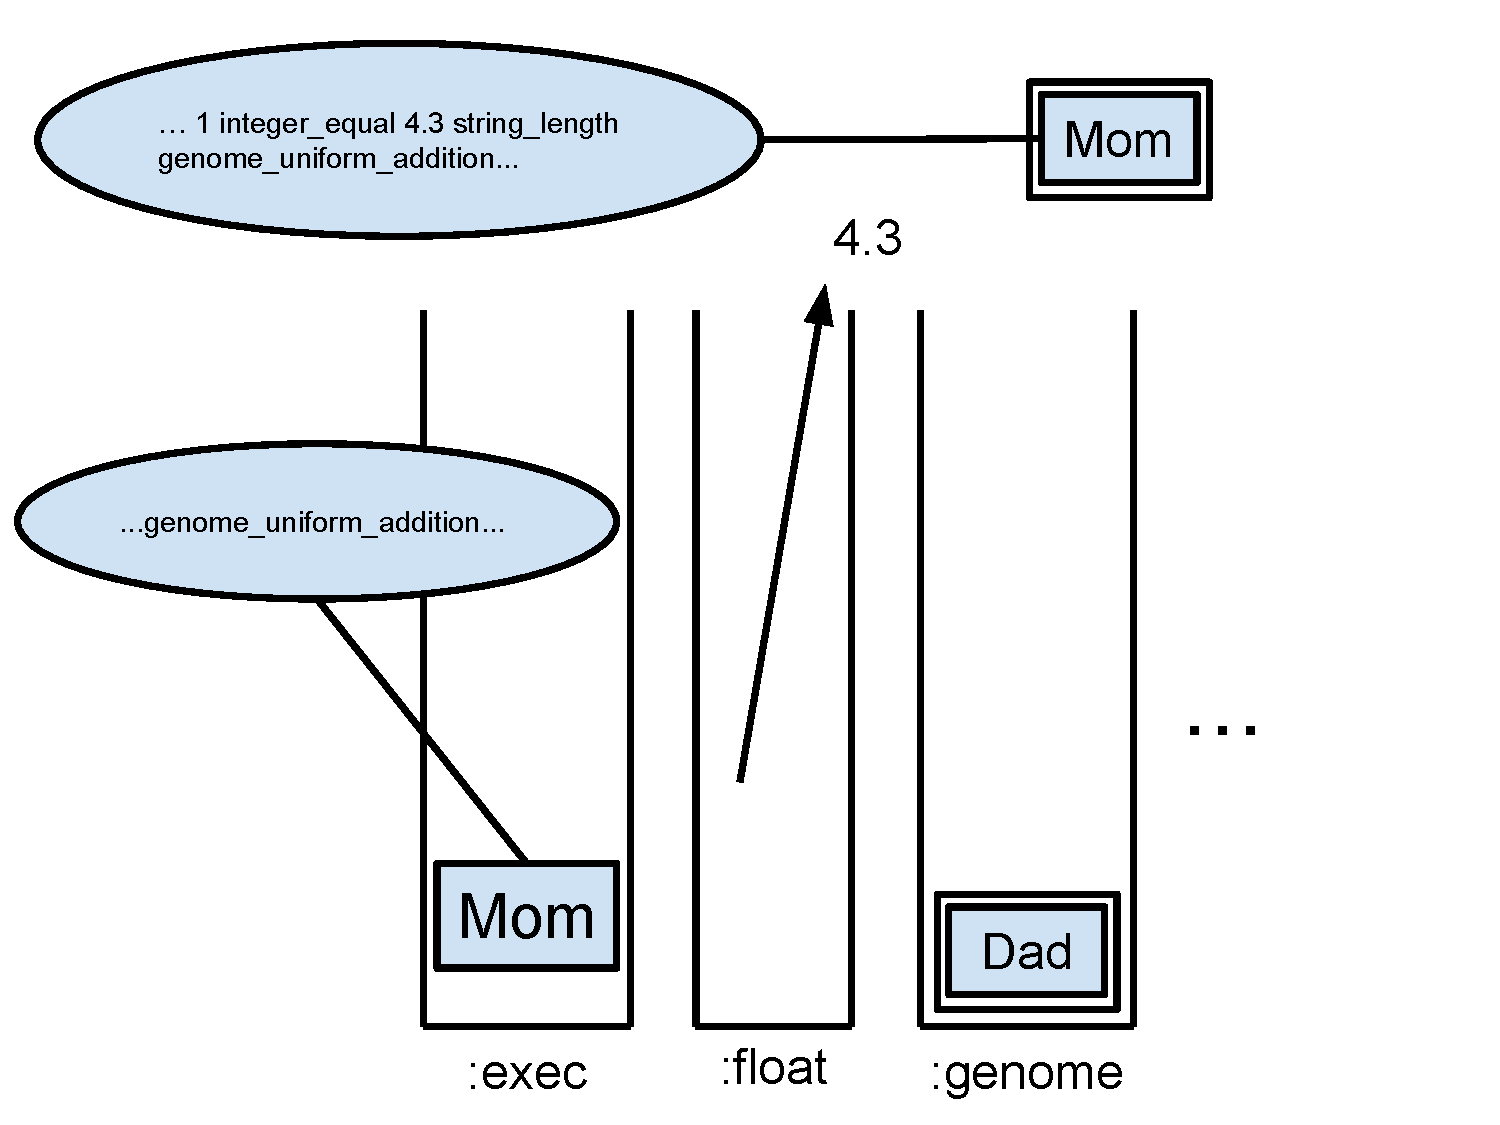
\includegraphics[width=.9\textwidth]{Illustrations/autodog_10.PDF}
\end{frame}

\begin{frame}
	\frametitle{AutoDoG~--~reproduction}
	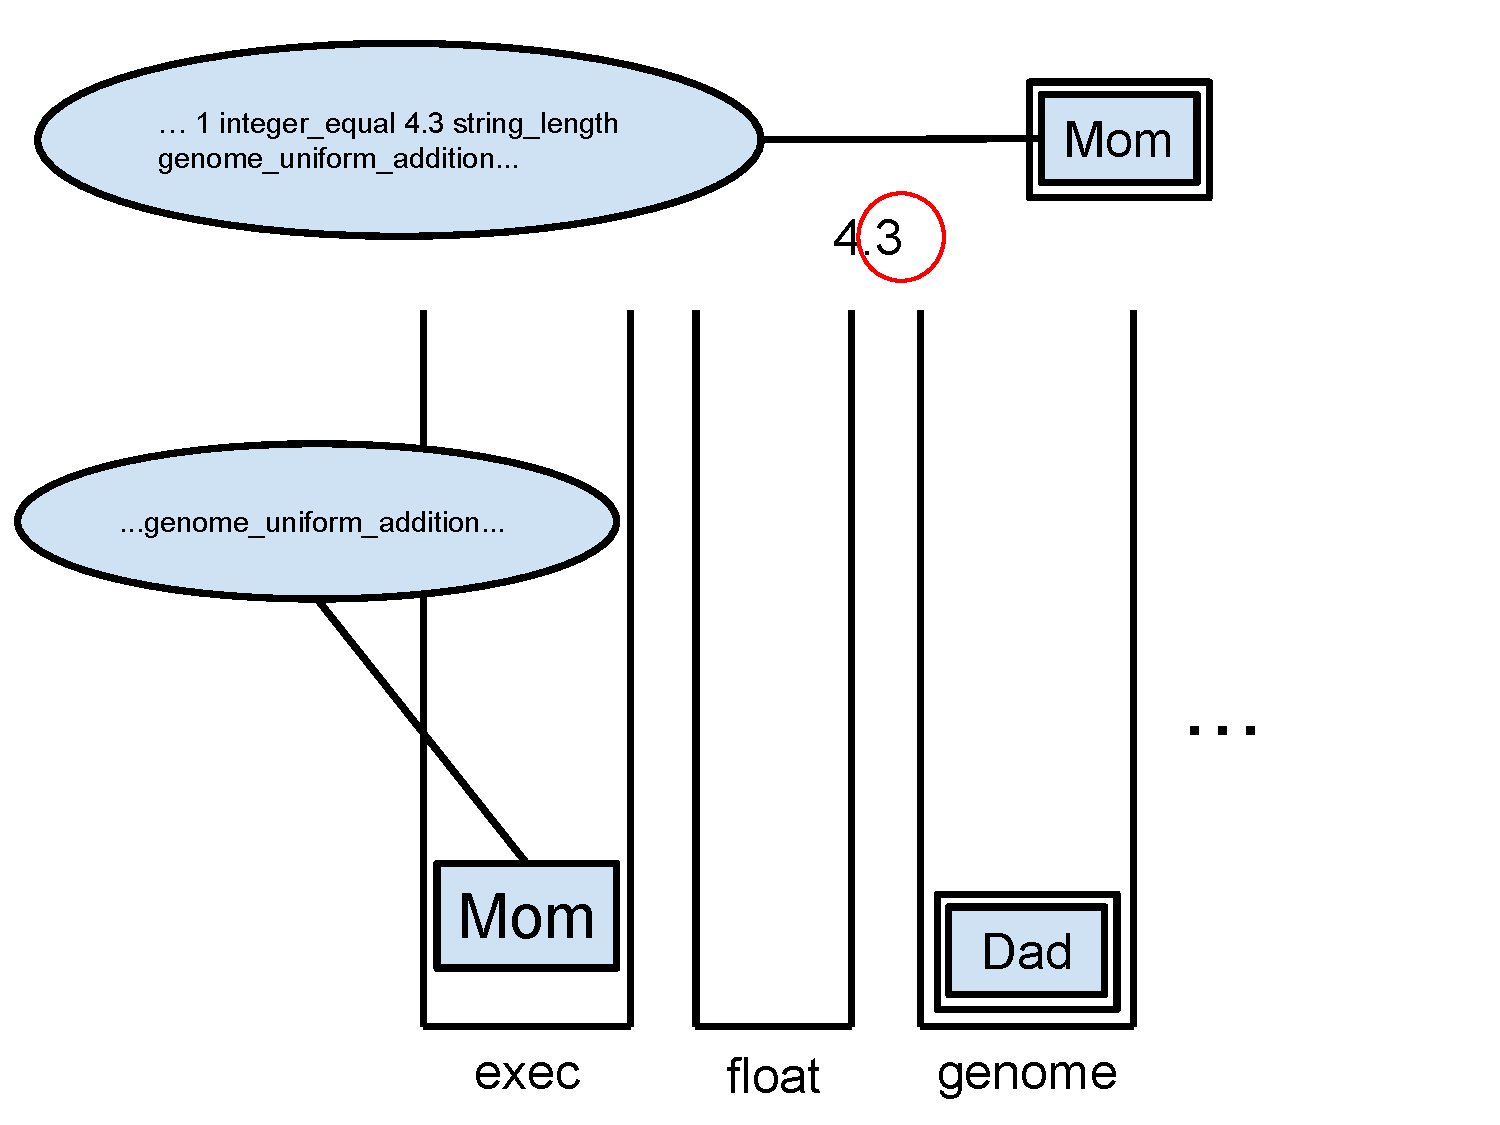
\includegraphics[width=.9\textwidth]{Illustrations/autodog_11.PDF}
\end{frame}

\begin{frame}
	\frametitle{AutoDoG~--~reproduction}
	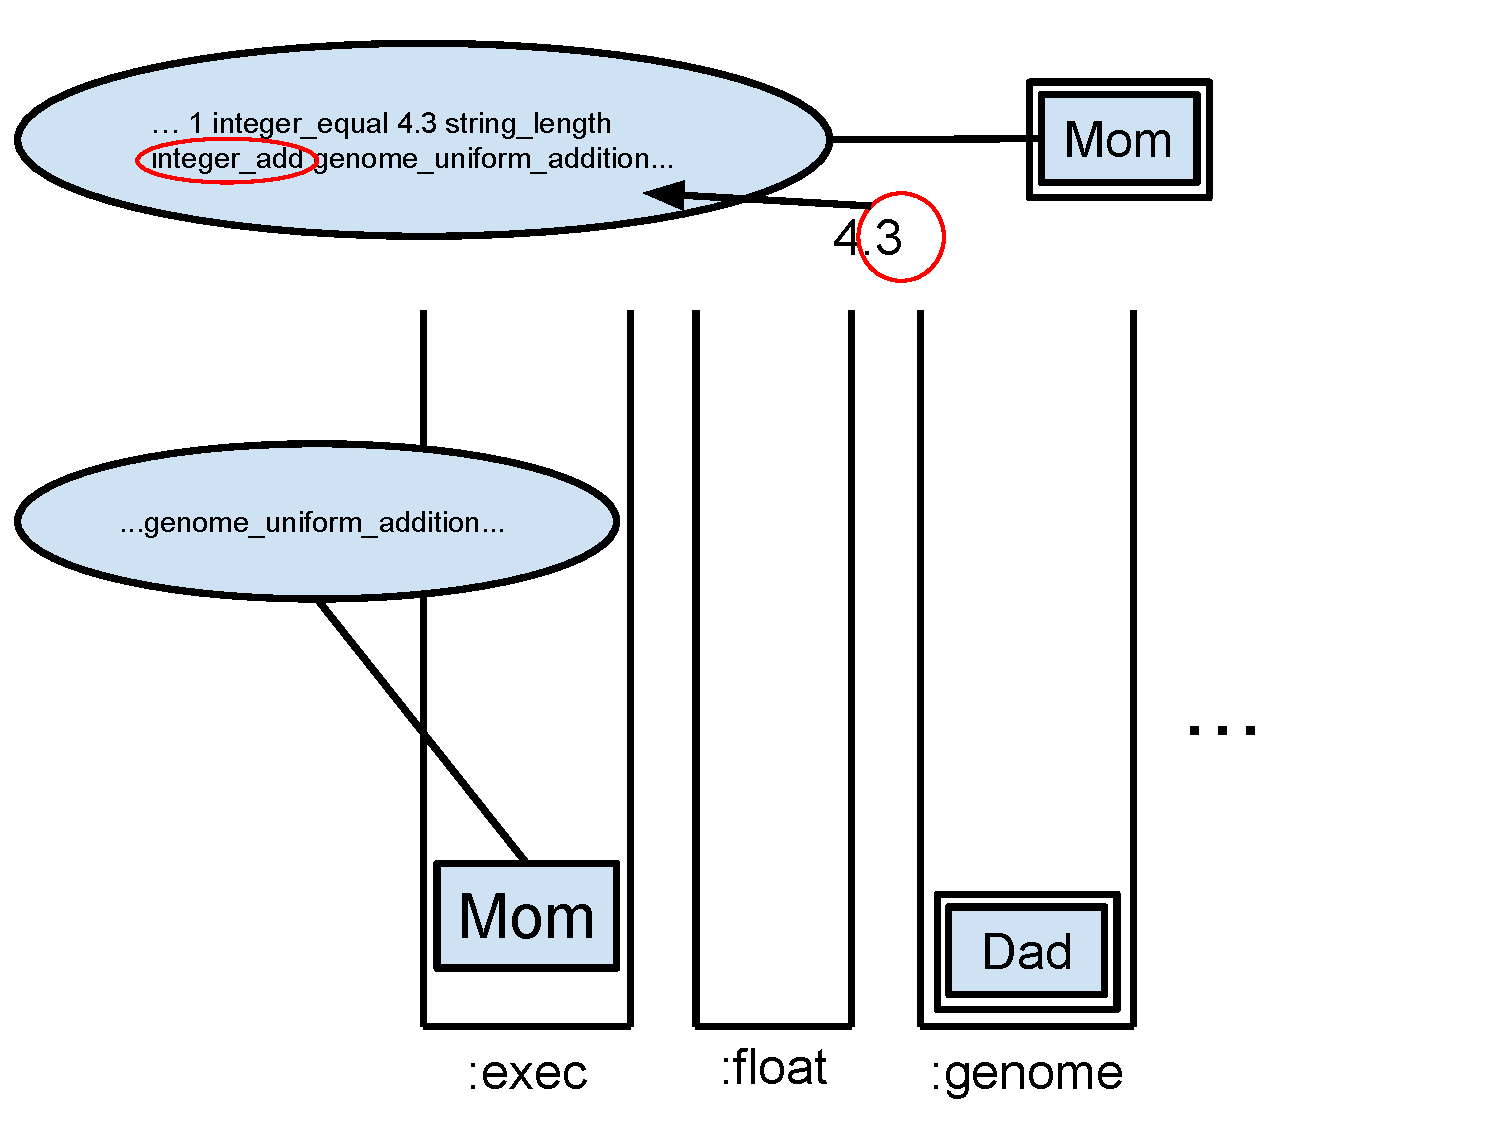
\includegraphics[width=.9\textwidth]{Illustrations/autodog_12.PDF}
\end{frame}

\begin{frame}
	\frametitle{AutoDoG~--~reproduction}
	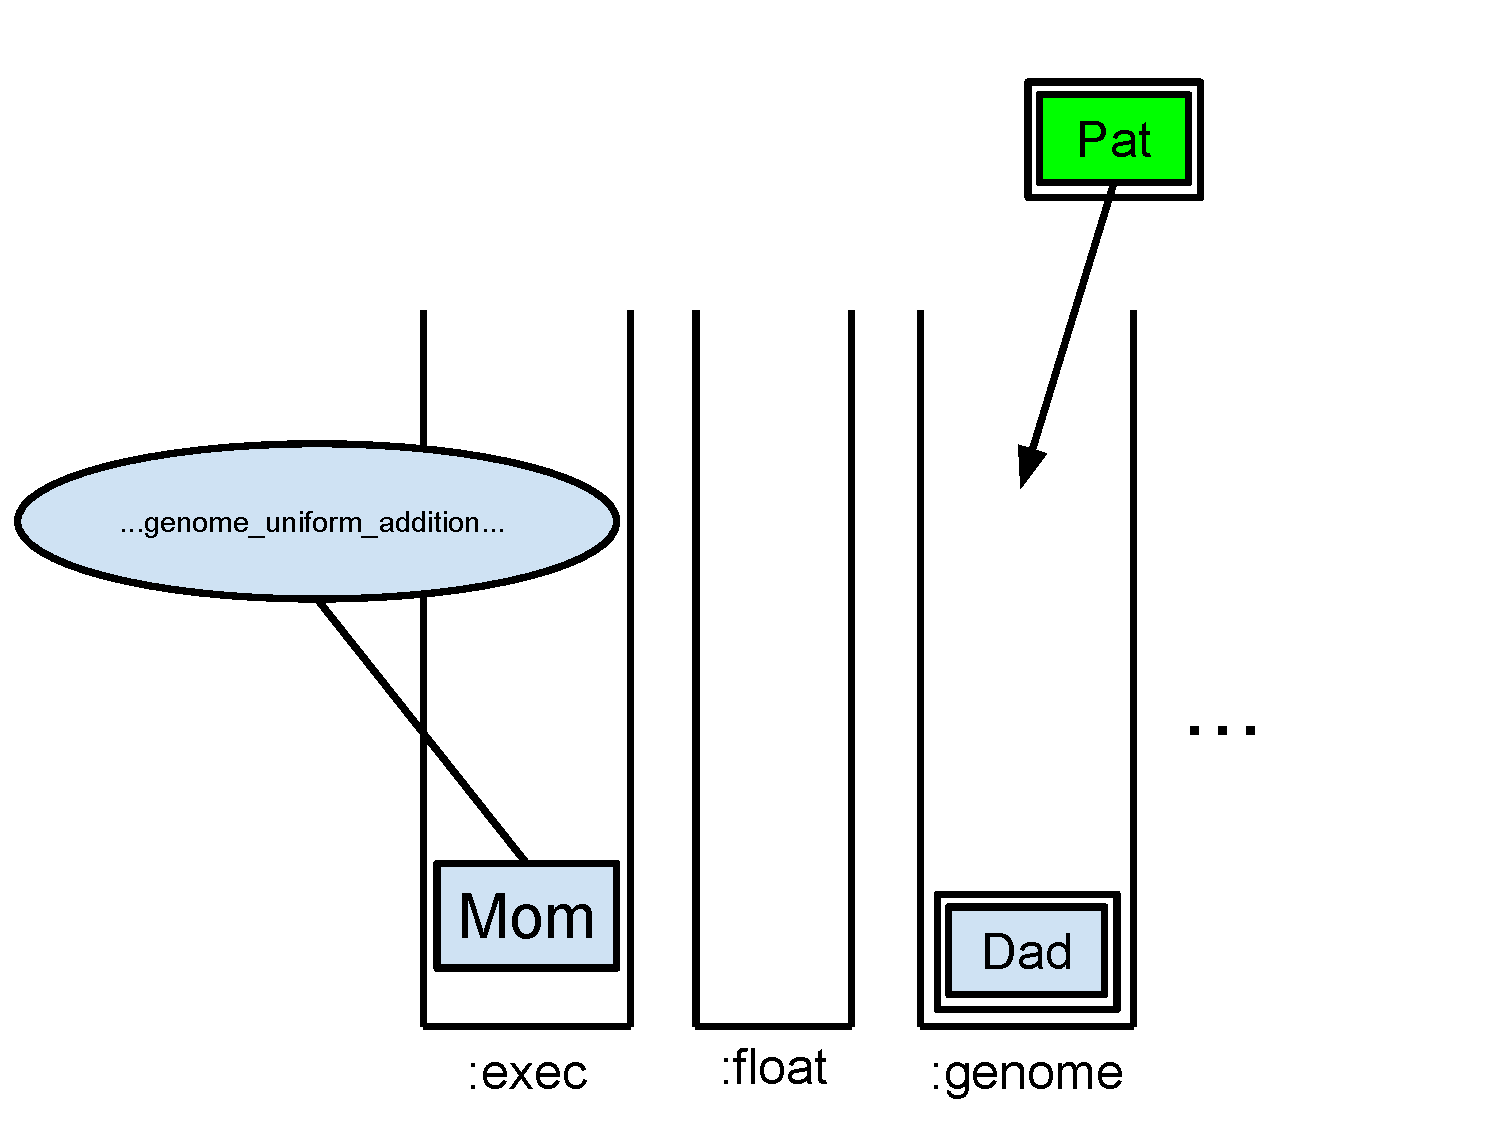
\includegraphics[width=.9\textwidth]{Illustrations/autodog_13.PDF}
\end{frame}

\begin{frame}
	\frametitle{AutoDoG~--~reproduction}
	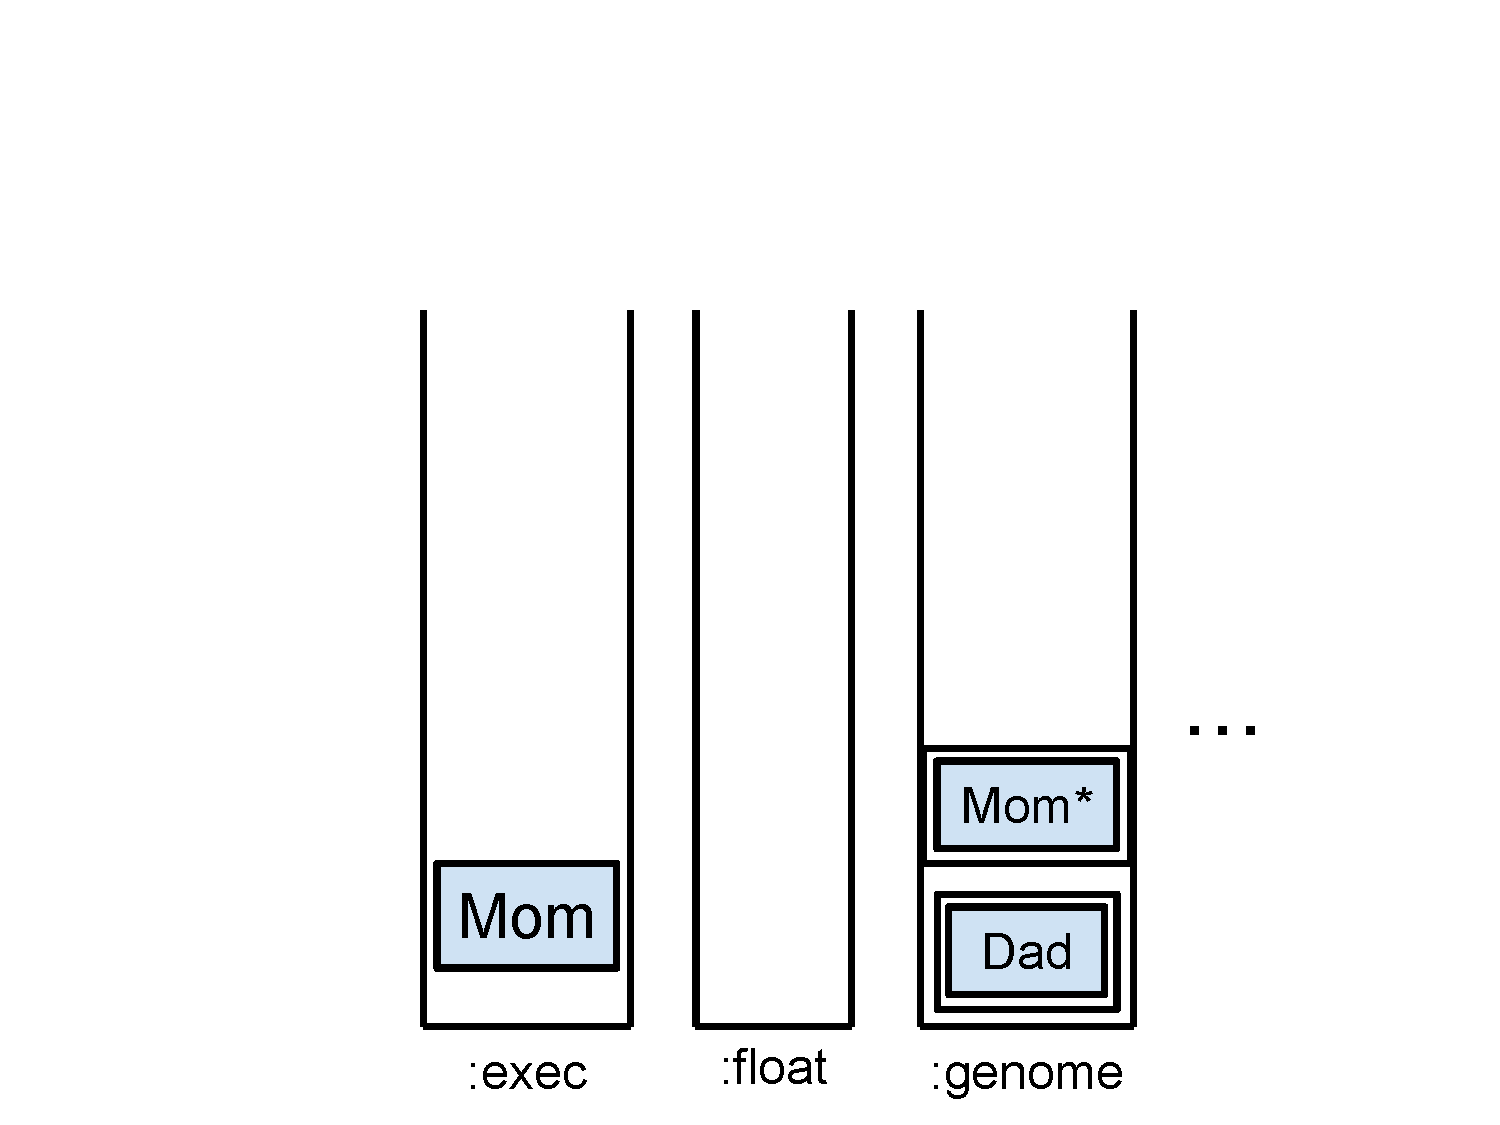
\includegraphics[width=.9\textwidth]{Illustrations/autodog_14.PDF}
\end{frame}
\begin{frame}
	\frametitle{AutoDoG~--~reproduction}
	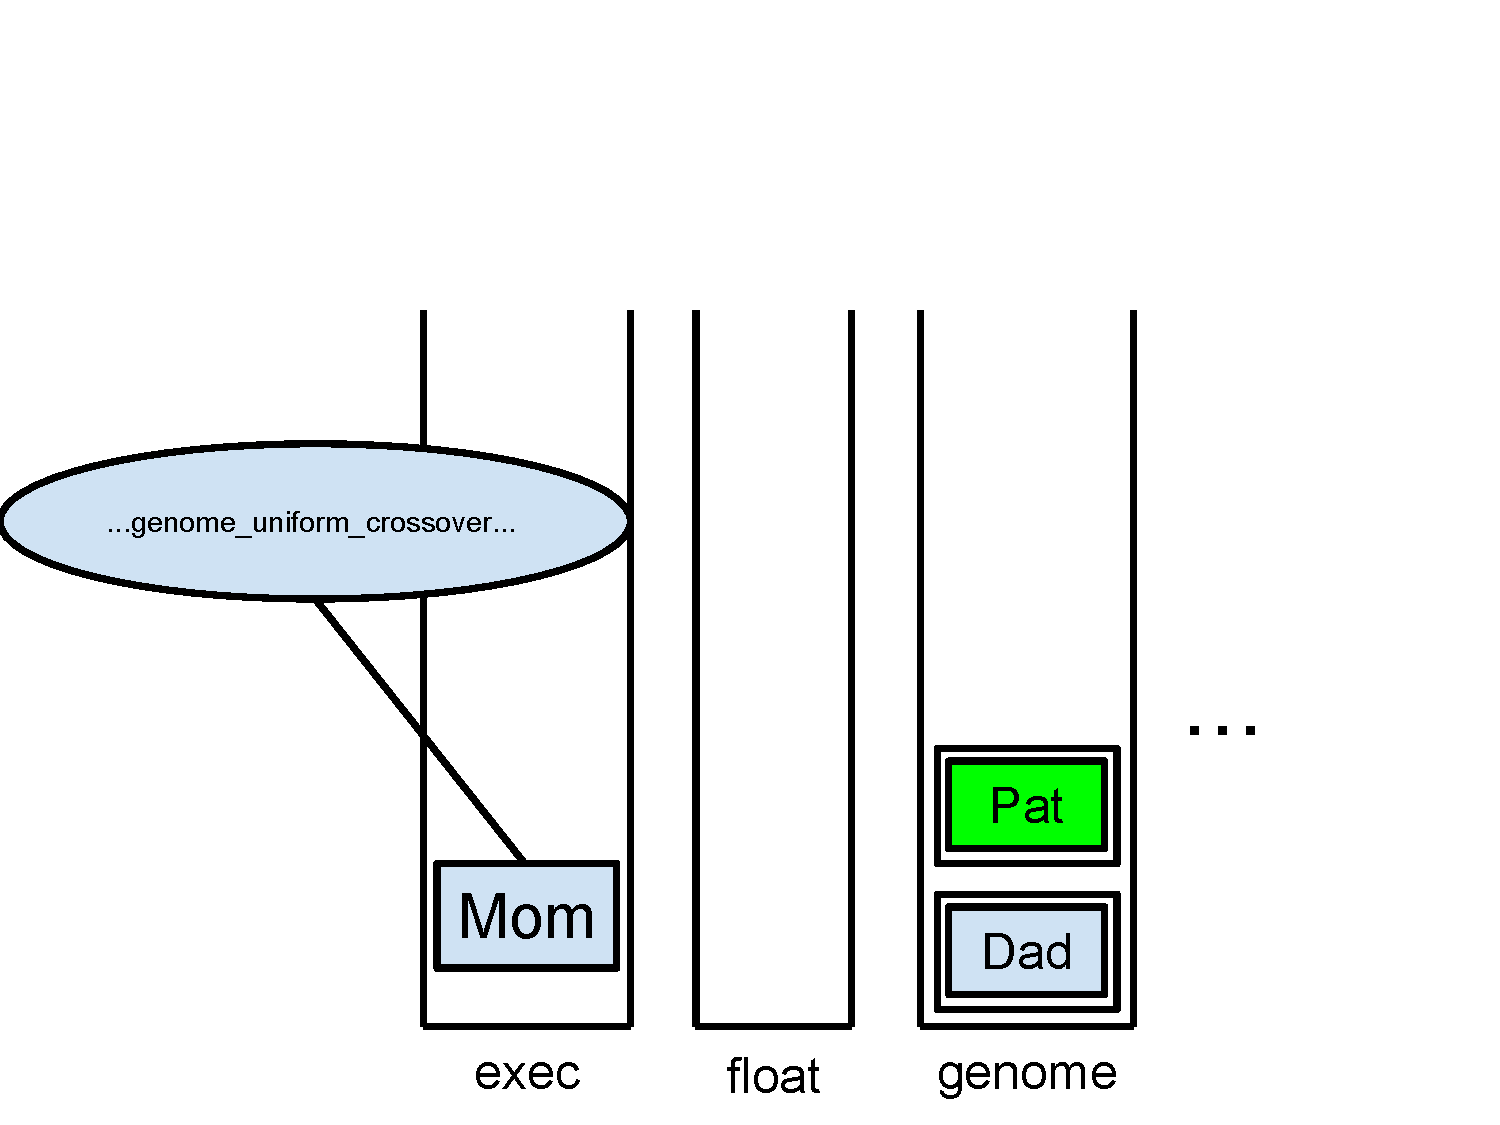
\includegraphics[width=.9\textwidth]{Illustrations/autodog_15.PDF}
\end{frame}

\begin{frame}
	\frametitle{AutoDoG~--~reproduction}
	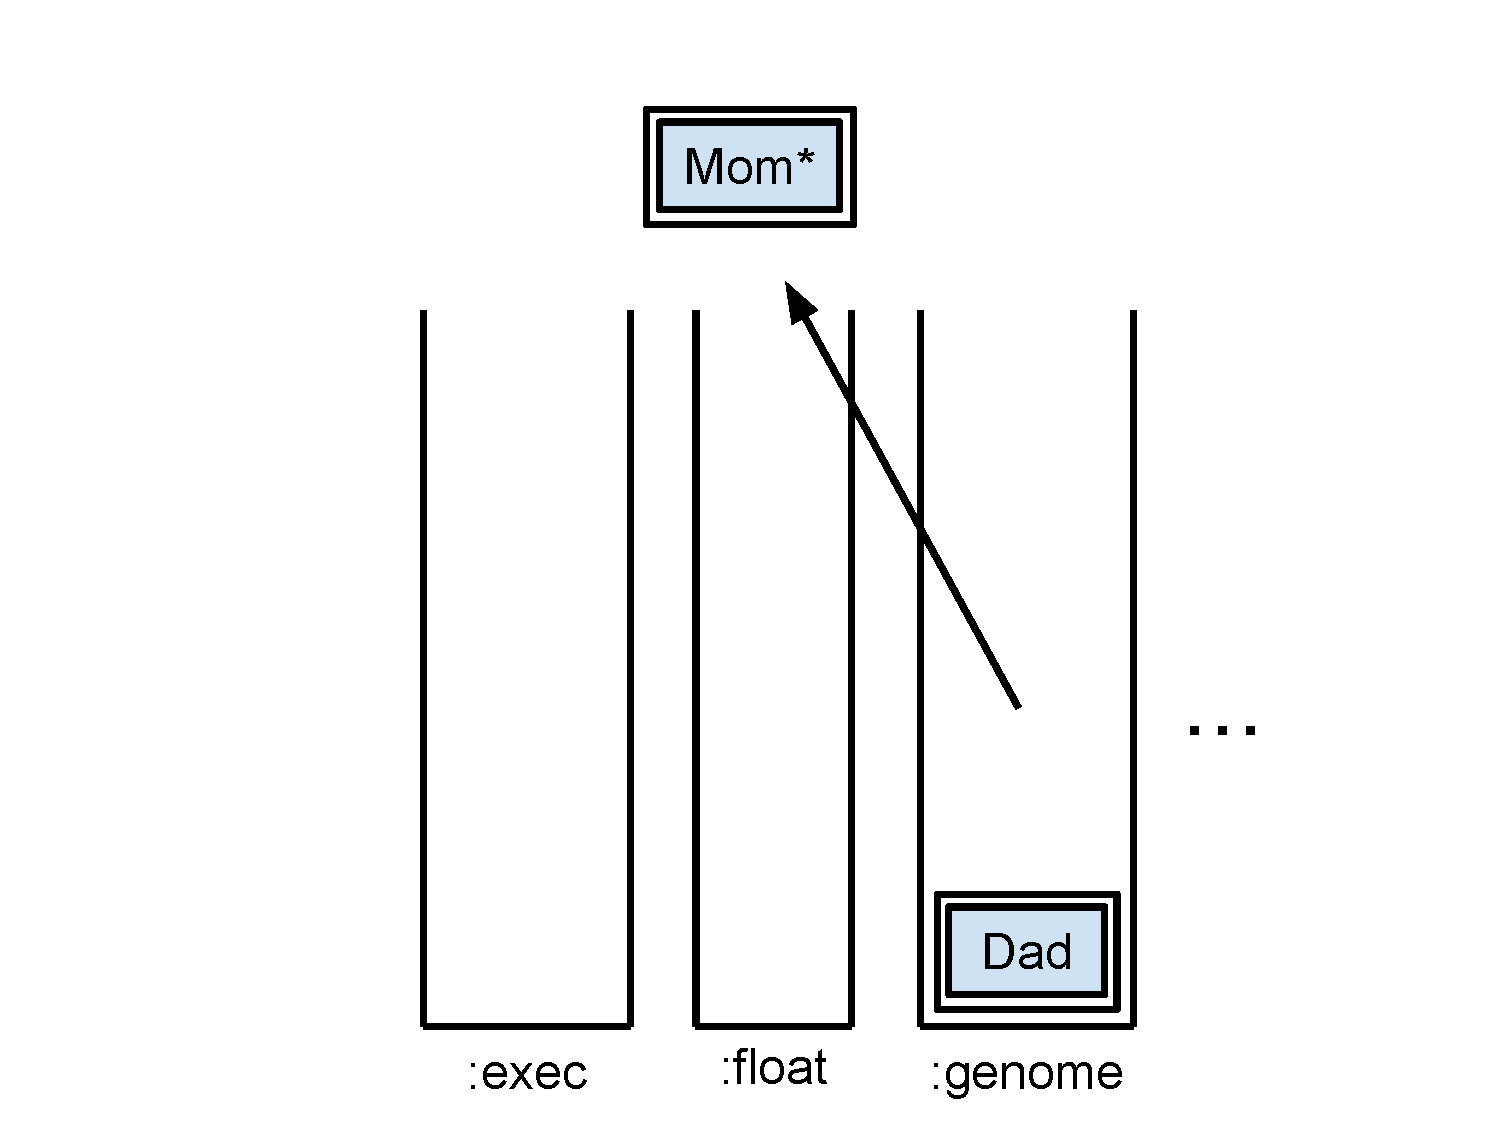
\includegraphics[width=.9\textwidth]{Illustrations/autodog_16.PDF}
\end{frame}

\begin{frame}
	\frametitle{AutoDoG~--~reproduction}
	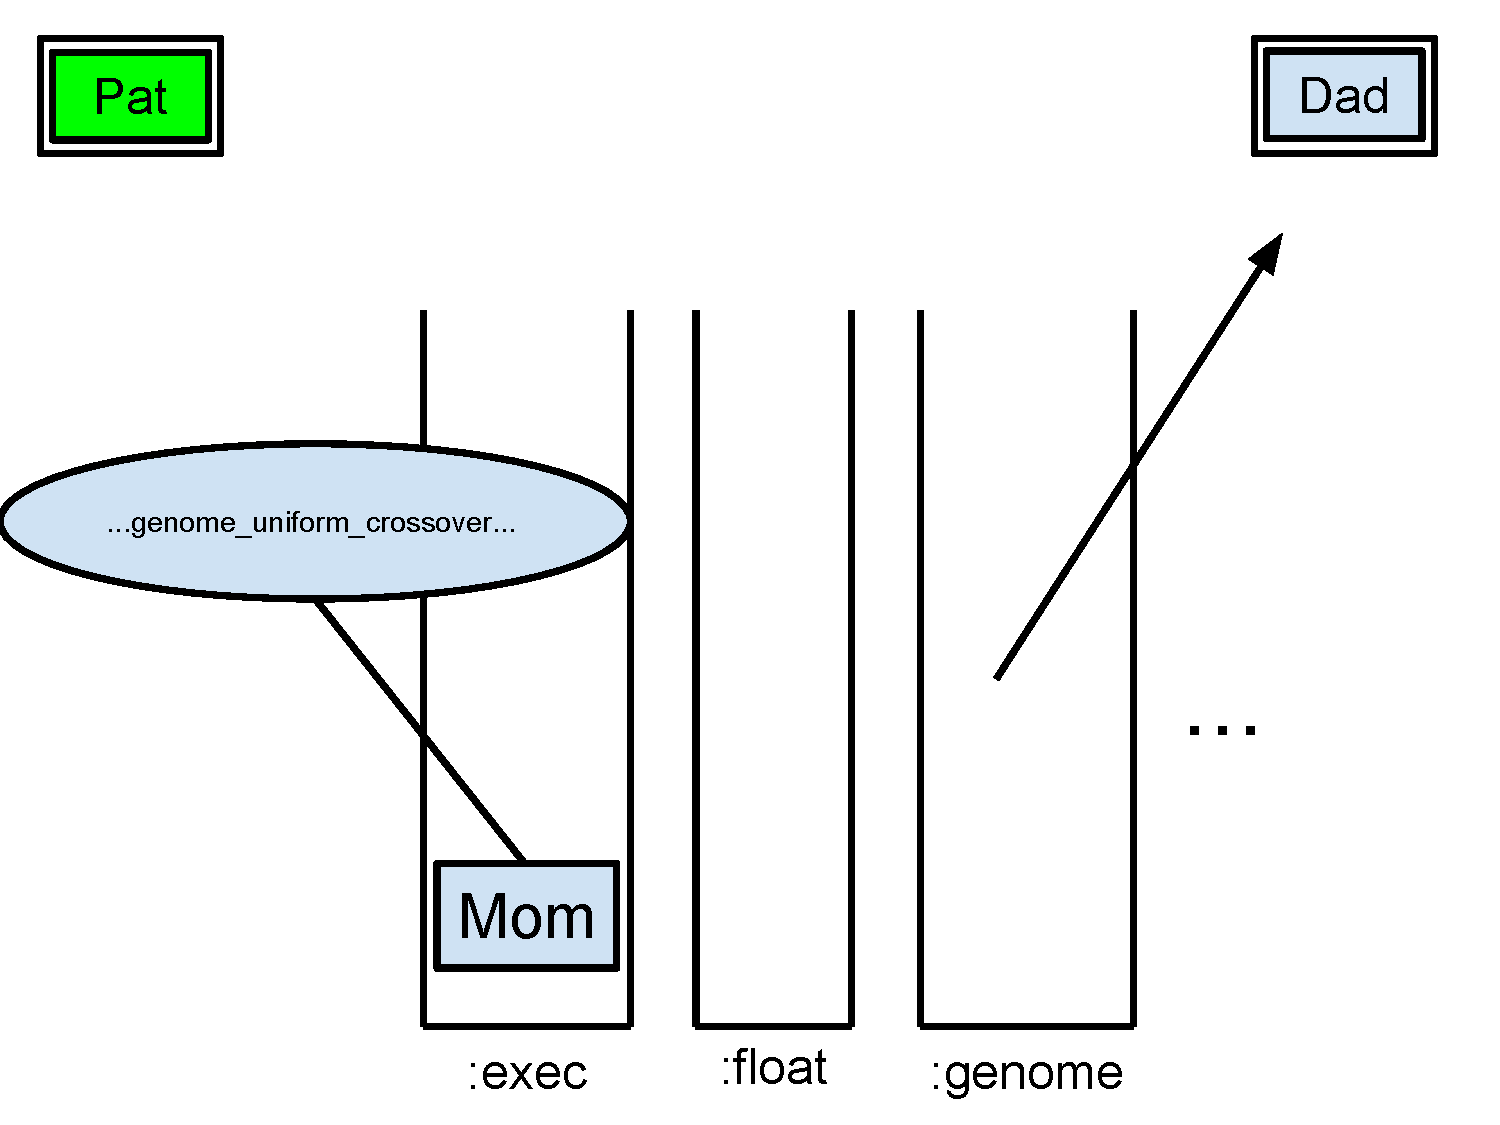
\includegraphics[width=.9\textwidth]{Illustrations/autodog_17.PDF}
\end{frame}

\begin{frame}
	\frametitle{AutoDoG~--~reproduction}
	\centering
	Now Child moves on to the next generation, right?
	\pause
	\linespace\linespace
	\large WRONG!
\end{frame}

\begin{frame}
	\frametitle{AutoDoG~--~diversification test}
	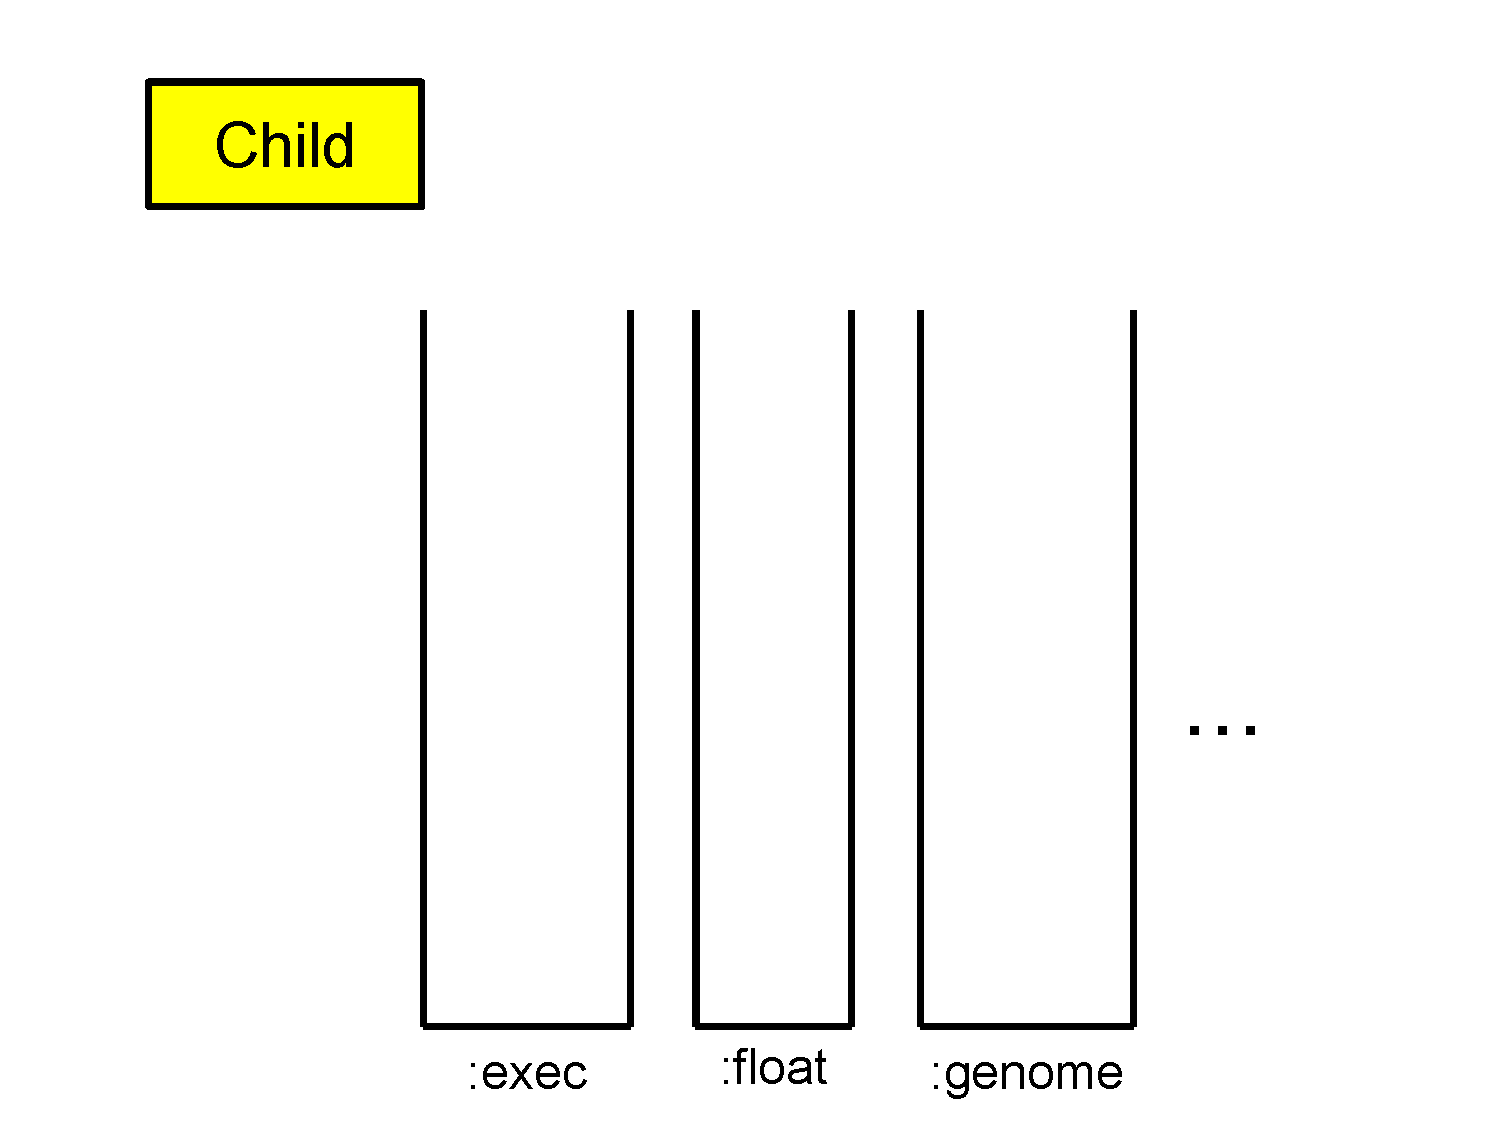
\includegraphics[width=.9\textwidth]{Illustrations/test_1.PDF}
\end{frame}

\begin{frame}
	\frametitle{AutoDoG~--~diversification test}
	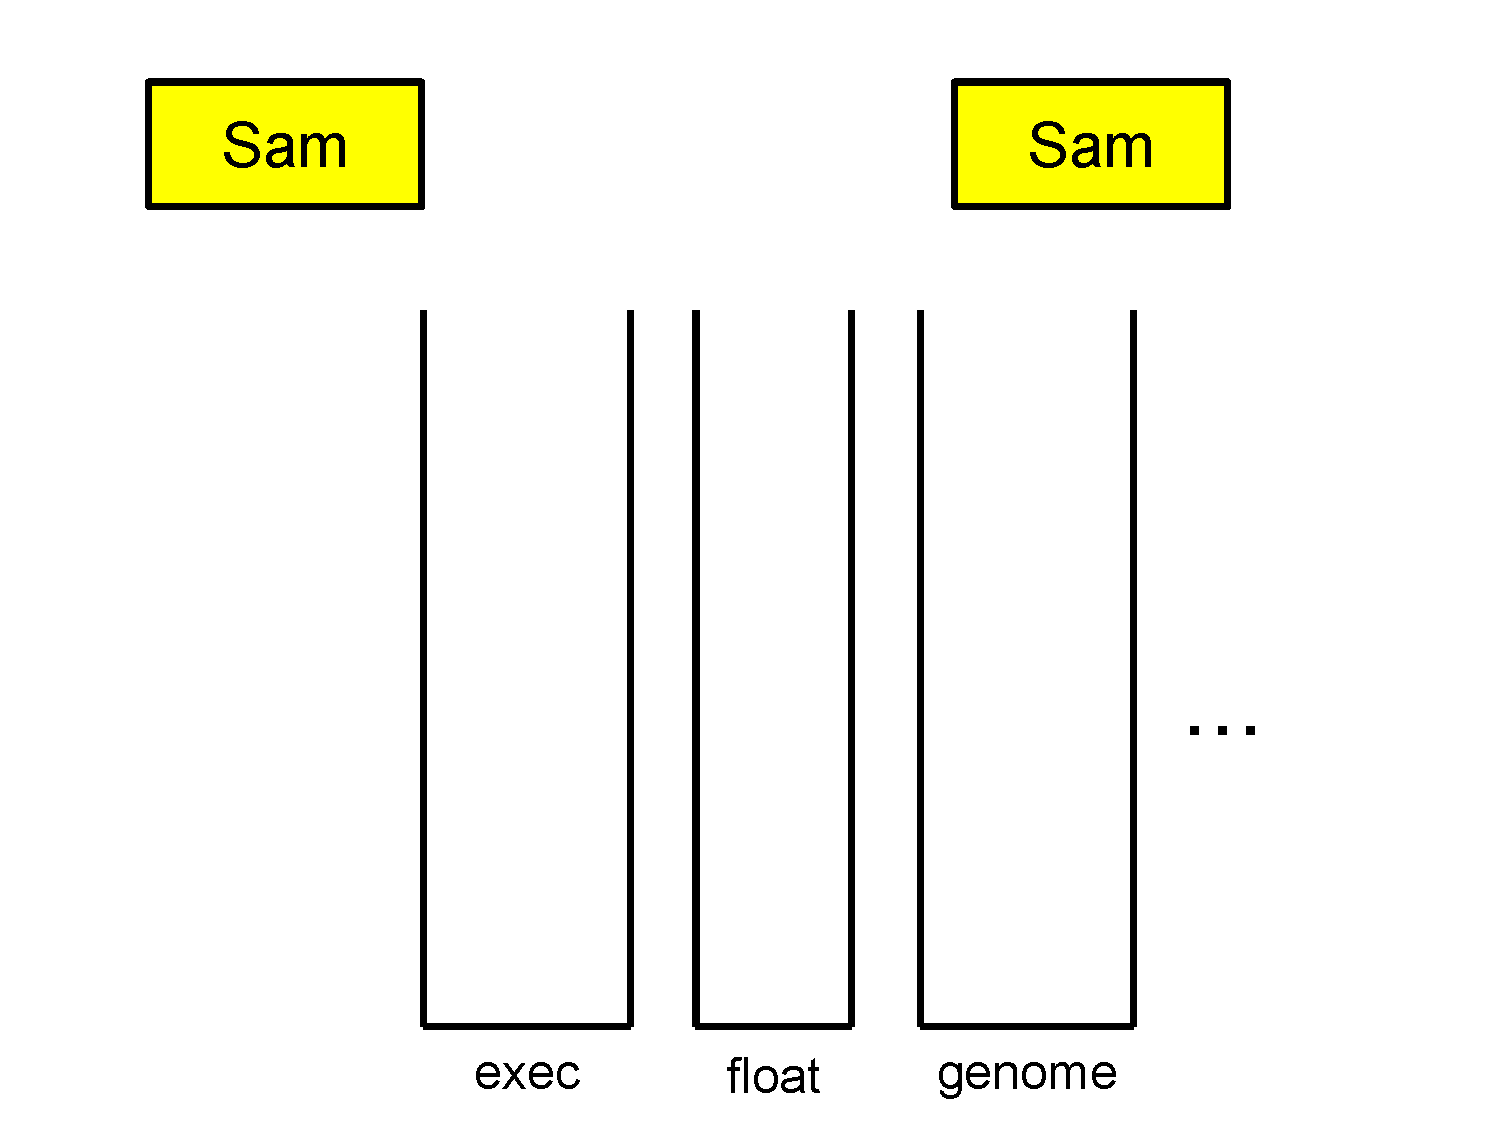
\includegraphics[width=.9\textwidth]{Illustrations/test_2.PDF}
\end{frame}

\begin{frame}
	\frametitle{AutoDoG~--~diversification test}
	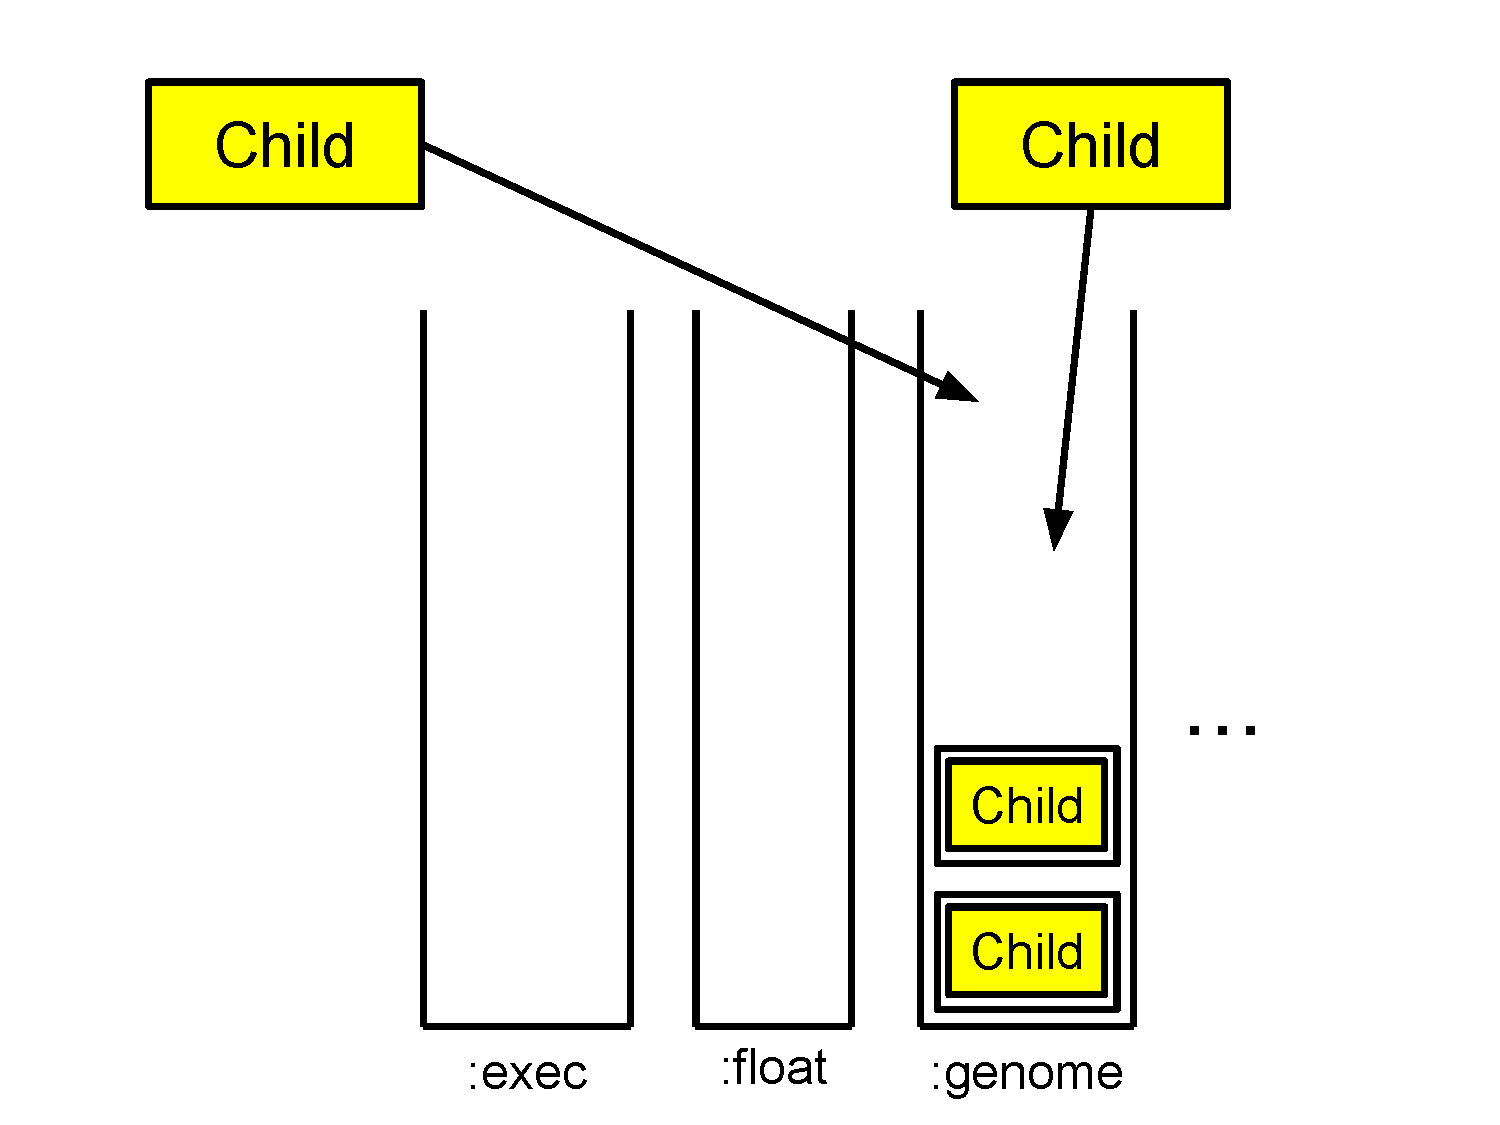
\includegraphics[width=.9\textwidth]{Illustrations/test_3.PDF}
\end{frame}

\begin{frame}
	\frametitle{AutoDoG~--~diversification test}
	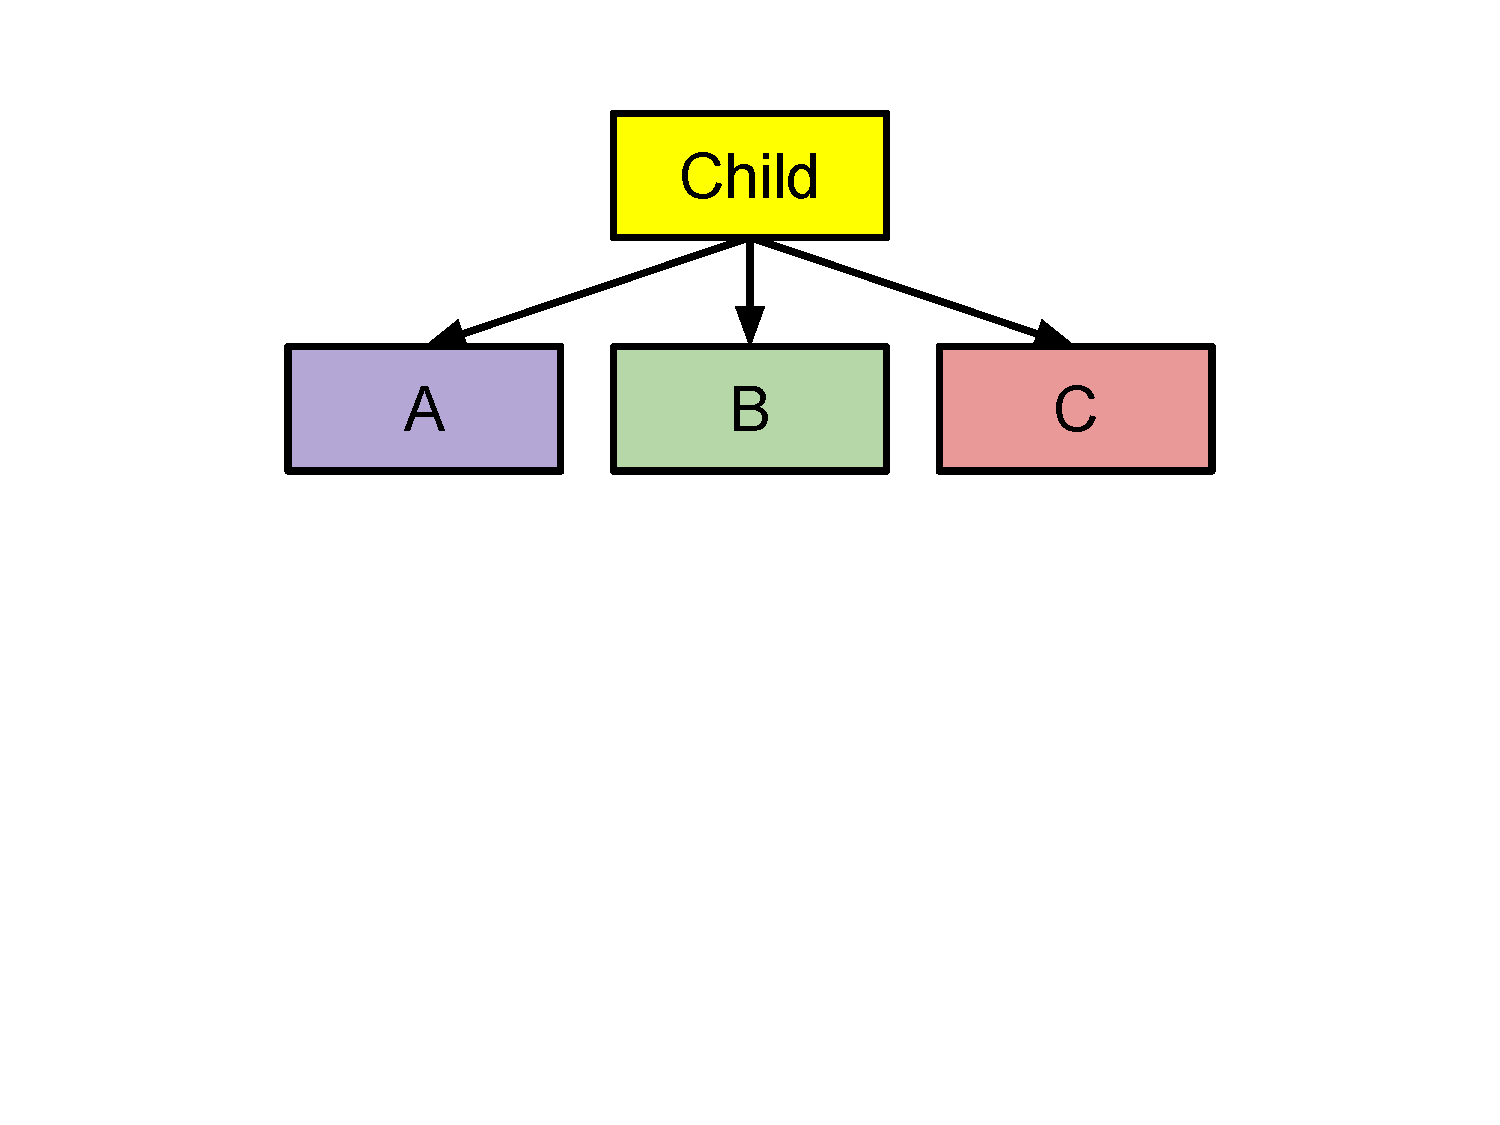
\includegraphics[width=.9\textwidth]{Illustrations/test_4.PDF}
\end{frame}

\begin{frame}
	\frametitle{AutoDoG~--~diversification test}
	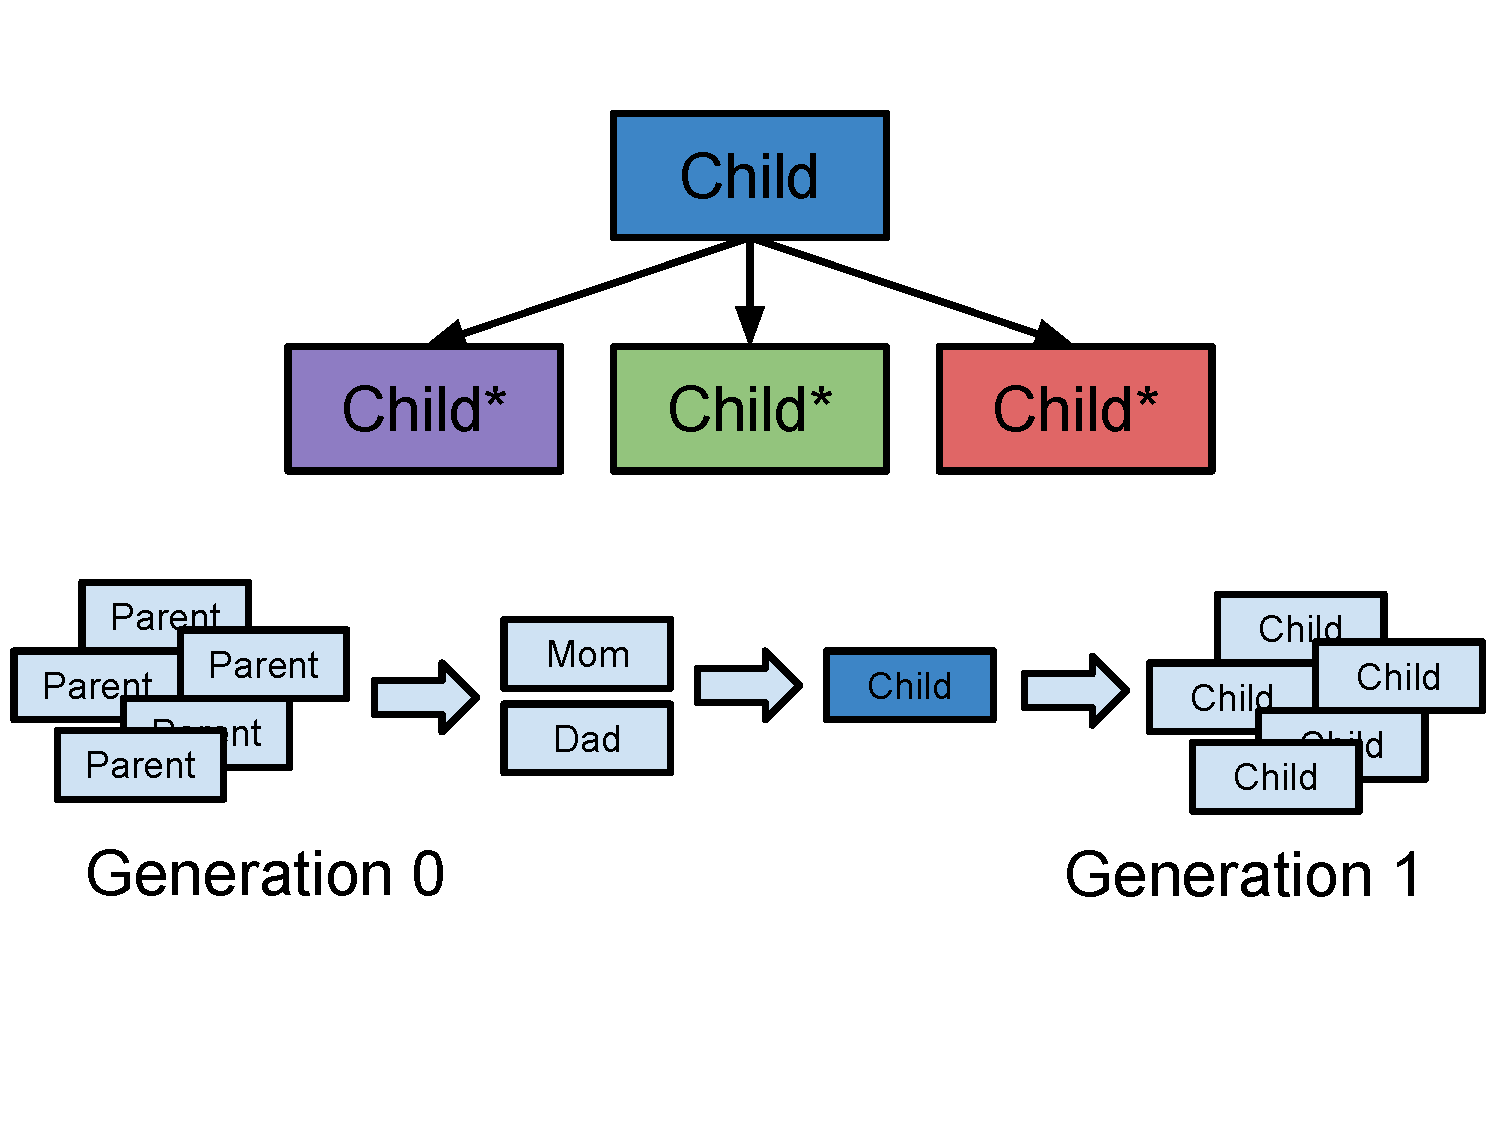
\includegraphics[width=.9\textwidth]{Illustrations/test_5.PDF}
\end{frame}

\begin{frame}
	\frametitle{AutoDoG~--~diversification test}
	\includegraphics[width=.9\textwidth]{Illustrations/test_6.PDF}
\end{frame}

\begin{frame}
	\frametitle{AutoDoG~--~diversification test}
	\includegraphics[width=.9\textwidth]{Illustrations/test_7.PDF}
\end{frame}

\begin{frame}
	\frametitle{AutoDoG~--~diversification test}
	\includegraphics[width=.9\textwidth]{Illustrations/test_8.PDF}
\end{frame}

\begin{frame}
	\frametitle{AutoDoG~--~diversification test}
	\includegraphics[width=.9\textwidth]{Illustrations/test_9.PDF}
\end{frame}

\begin{frame}
	\frametitle{AutoDoG~--~diversification test}
	\includegraphics[width=.9\textwidth]{Illustrations/test_10.PDF}
\end{frame}

\subsection{Results of AutoDoG}

\section[Summary]{Summary}

\begin{frame} 
	\frametitle{References} 
	
	\begin{thebibliography}{lskdjf}
		
		\bibitem{harris:2015}
		S.~Harris, T.~Bueter, and D.~R.~Tauritz.
		\newblock A Comparison of Genetic Programming Variants for Hyper-Heuristics.
		\newblock In Sara~Silva, editors, {\em GECCO '15}, pages 1043--1050, Madrid, Spain 2015.
		
		\bibitem{spector:2016}
		L.~Spector, N.~F.~McPhee, T.~Helmuth, M.~M.~Casale, and J.~Oks.
		\newblock Evolution Evolves with Autoconstruction.
		\newblock In T.~Friedrich, \emph{et al}, editors, {\em GECCO '16}, pages 1349--1356, Denver, Colorado, USA 2016.
		
	\end{thebibliography}
	
	\linespace
	\begin{center}
		See my paper for additional references.
	\end{center}
\end{frame} 

\end{document}


\end{document}